%%%%%%%%%%%%%%%%%%%%%%%%%%%%%%%%%%%%%%%%%
%  My documentation report
%  Objetive: Explain what I did and how, so someone can continue with the investigation
%
% Important note:
% Chapter heading images should have a 2:1 width:height ratio,
% e.g. 920px width and 460px height.
%
%%%%%%%%%%%%%%%%%%%%%%%%%%%%%%%%%%%%%%%%%

%----------------------------------------------------------------------------------------
%	PACKAGES AND OTHER DOCUMENT CONFIGURATIONS
%----------------------------------------------------------------------------------------

\documentclass[12pt,ngerman, fleqn]{book} % Default font size and left-justified equations

\usepackage[top=3cm,bottom=3cm,left=3.2cm,right=3.2cm,headsep=10pt,letterpaper]{geometry} % Page margins

\usepackage{xcolor} % Required for specifying colors by name
\definecolor{ocre}{RGB}{52,177,201} % Define the orange color used for highlighting throughout the book

%Imojis :)
%\usepackage{coloremoji}

%Euro sign
\usepackage{german}
\usepackage{eurosym}

%figure wrap
\usepackage{wrapfig}

%Special charachters
\usepackage{pifont}

%add apendix
\usepackage[toc,page]{appendix}

% spalten listen
\usepackage{blindtext}
\usepackage{tasks}

% for figure grouping
\usepackage{subcaption}
\usepackage{graphicx}

% Font Settings
\usepackage{avant} % Use the Avantgarde font for headings
%\usepackage{times} % Use the Times font for headings
\usepackage{mathptmx} % Use the Adobe Times Roman as the default text font together with math symbols from the Symbol, Chancery and Computer Modern fonts

%\usepackage{microtype} % Slightly tweak font spacing for aesthetics
\usepackage[utf8]{inputenc} % Required for including letters with accents 
\usepackage[T1]{fontenc} % Use 8-bit encoding that has 256 glyphs

% Bibliography
%\usepackage[style=alphabetic,sorting=nyt,sortcites=true,autopunct=true,babel=hyphen,hyperref=true,abbreviate=false,backref=true,backend=biber]{biblatex}
%\addbibresource{bibliography.bib} % BibTeX bibliography file
%\defbibheading{bibempty}{}

\usepackage{csquotes}
\usepackage[style=verbose-ibid,backend=bibtex]{biblatex}
\addbibresource{bibliography.bib}

%----------------------------------------------------------------------------------------
%	VARIOUS REQUIRED PACKAGES
%----------------------------------------------------------------------------------------

\usepackage{titlesec} % Allows customization of titles

\usepackage{graphicx} % Required for including pictures
\graphicspath{{Pictures/}} % Specifies the directory where pictures are stored

\usepackage{lipsum} % Inserts dummy text

\usepackage{tikz} % Required for drawing custom shapes

\usepackage[german, english]{babel} % English language/hyphenation

\usepackage{enumitem} % Customize lists
\setlist{nolistsep} % Reduce spacing between bullet points and numbered lists

\usepackage{booktabs} % Required for nicer horizontal rules in tables

\usepackage{eso-pic} % Required for specifying an image background in the title page

%----------------------------------------------------------------------------------------
%	MAIN TABLE OF CONTENTS
%----------------------------------------------------------------------------------------

\usepackage{titletoc} % Required for manipulating the table of contents

\contentsmargin{0cm} % Removes the default margin
% Chapter text styling
\titlecontents{chapter}[1.25cm] % Indentation
{\addvspace{15pt}\large\sffamily\bfseries} % Spacing and font options for chapters
{\color{ocre!60}\contentslabel[\Large\thecontentslabel]{1.25cm}\color{ocre}} % Chapter number
{}  
{\color{ocre!60}\normalsize\sffamily\bfseries\;\titlerule*[.5pc]{.}\;\thecontentspage} % Page number
% Section text styling
\titlecontents{section}[1.25cm] % Indentation
{\addvspace{5pt}\sffamily\bfseries} % Spacing and font options for sections
{\contentslabel[\thecontentslabel]{1.25cm}} % Section number
{}
{\sffamily\hfill\color{black}\thecontentspage} % Page number
[]
% Subsection text styling
\titlecontents{subsection}[1.25cm] % Indentation
{\addvspace{1pt}\sffamily\small} % Spacing and font options for subsections
{\contentslabel[\thecontentslabel]{1.25cm}} % Subsection number
{}
{\sffamily\;\titlerule*[.5pc]{.}\;\thecontentspage} % Page number
[] 

\setcounter{page}{-2}

%----------------------------------------------------------------------------------------
%	MINI TABLE OF CONTENTS IN CHAPTER HEADS
%----------------------------------------------------------------------------------------

%noindention
\setlength\parindent{0pt}

% Section text styling
\titlecontents{lsection}[0em] % Indendating
{\footnotesize\sffamily} % Font settings
{}
{}
{}

% Subsection text styling
\titlecontents{lsubsection}[.5em] % Indentation
{\normalfont\footnotesize\sffamily} % Font settings
{}
{}
{}
 
%----------------------------------------------------------------------------------------
%	PAGE HEADERS
%----------------------------------------------------------------------------------------

\usepackage{fancyhdr} % Required for header and footer configuration

\pagestyle{fancy}
\renewcommand{\chaptermark}[1]{\markboth{\sffamily\normalsize\bfseries\chaptername\ \thechapter.\ #1}{}} % Chapter text font settings
\renewcommand{\sectionmark}[1]{\markright{\sffamily\normalsize\thesection\hspace{5pt}#1}{}} % Section text font settings
\fancyhf{} \fancyhead[LE,RO]{\sffamily\normalsize\thepage} % Font setting for the page number in the header
\fancyhead[LO]{\rightmark} % Print the nearest section name on the left side of odd pages
\fancyhead[RE]{\leftmark} % Print the current chapter name on the right side of even pages
\renewcommand{\headrulewidth}{0.5pt} % Width of the rule under the header
\addtolength{\headheight}{2.5pt} % Increase the spacing around the header slightly
\renewcommand{\footrulewidth}{0pt} % Removes the rule in the footer
\fancypagestyle{plain}{\fancyhead{}\renewcommand{\headrulewidth}{0pt}} % Style for when a plain pagestyle is specified

% Removes the header from odd empty pages at the end of chapters
\makeatletter
\renewcommand{\cleardoublepage}{
\clearpage\ifodd\c@page\else
\hbox{}
\vspace*{\fill}
\thispagestyle{empty}
\newpage
\fi}

%----------------------------------------------------------------------------------------
%	THEOREM STYLES
%----------------------------------------------------------------------------------------

\usepackage{amsmath,amsfonts,amssymb,amsthm} % For math equations, theorems, symbols, etc

\newcommand{\intoo}[2]{\mathopen{]}#1\,;#2\mathclose{[}}
\newcommand{\ud}{\mathop{\mathrm{{}d}}\mathopen{}}
\newcommand{\intff}[2]{\mathopen{[}#1\,;#2\mathclose{]}}
\newtheorem{notation}{Notation}[chapter]

%%%%%%%%%%%%%%%%%%%%%%%%%%%%%%%%%%%%%%%%%%%%%%%%%%%%%%%%%%%%%%%%%%%%%%%%%%%
%%%%%%%%%%%%%%%%%%%% dedicated to boxed/framed environements %%%%%%%%%%%%%%
%%%%%%%%%%%%%%%%%%%%%%%%%%%%%%%%%%%%%%%%%%%%%%%%%%%%%%%%%%%%%%%%%%%%%%%%%%%
\newtheoremstyle{ocrenumbox}% % Theorem style name
{0pt}% Space above
{0pt}% Space below
{\normalfont}% % Body font
{}% Indent amount
{\small\bf\sffamily\color{ocre}}% % Theorem head font
{\;}% Punctuation after theorem head
{0.25em}% Space after theorem head
{\small\sffamily\color{ocre}\thmname{#1}\nobreakspace\thmnumber{\@ifnotempty{#1}{}\@upn{#2}}% Theorem text (e.g. Theorem 2.1)
\thmnote{\nobreakspace\the\thm@notefont\sffamily\bfseries\color{black}---\nobreakspace#3.}} % Optional theorem note
\renewcommand{\qedsymbol}{$\blacksquare$}% Optional qed square

\newtheoremstyle{blacknumex}% Theorem style name
{5pt}% Space above
{5pt}% Space below
{\normalfont}% Body font
{} % Indent amount
{\small\bf\sffamily}% Theorem head font
{\;}% Punctuation after theorem head
{0.25em}% Space after theorem head
{\small\sffamily{\tiny\ensuremath{\blacksquare}}\nobreakspace\thmname{#1}\nobreakspace\thmnumber{\@ifnotempty{#1}{}\@upn{#2}}% Theorem text (e.g. Theorem 2.1)
\thmnote{\nobreakspace\the\thm@notefont\sffamily\bfseries---\nobreakspace#3.}}% Optional theorem note

\newtheoremstyle{blacknumbox} % Theorem style name
{0pt}% Space above
{0pt}% Space below
{\normalfont}% Body font
{}% Indent amount
{\small\bf\sffamily}% Theorem head font
{\;}% Punctuation after theorem head
{0.25em}% Space after theorem head
{\small\sffamily\thmname{#1}\nobreakspace\thmnumber{\@ifnotempty{#1}{}\@upn{#2}}% Theorem text (e.g. Theorem 2.1)
\thmnote{\nobreakspace\the\thm@notefont\sffamily\bfseries---\nobreakspace#3.}}% Optional theorem note

%%%%%%%%%%%%%%%%%%%%%%%%%%%%%%%%%%%%%%%%%%%%%%%%%%%%%%%%%%%%%%%%%%%%%%%%%%%
%%%%%%%%%%%%% dedicated to non-boxed/non-framed environements %%%%%%%%%%%%%
%%%%%%%%%%%%%%%%%%%%%%%%%%%%%%%%%%%%%%%%%%%%%%%%%%%%%%%%%%%%%%%%%%%%%%%%%%%
\newtheoremstyle{ocrenum}% % Theorem style name
{5pt}% Space above
{5pt}% Space below
{\normalfont}% % Body font
{}% Indent amount
{\small\bf\sffamily\color{ocre}}% % Theorem head font
{\;}% Punctuation after theorem head
{0.25em}% Space after theorem head
{\small\sffamily\color{ocre}\thmname{#1}\nobreakspace\thmnumber{\@ifnotempty{#1}{}\@upn{#2}}% Theorem text (e.g. Theorem 2.1)
\thmnote{\nobreakspace\the\thm@notefont\sffamily\bfseries\color{black}---\nobreakspace#3.}} % Optional theorem note
\renewcommand{\qedsymbol}{$\blacksquare$}% Optional qed square
\makeatother

% Defines the theorem text style for each type of theorem to one of the three styles above
\newcounter{dummy} 
\numberwithin{dummy}{section}
\theoremstyle{ocrenumbox}
\newtheorem{theoremeT}[dummy]{Theorem}
\newtheorem{problem}{Problem}[chapter]
\newtheorem{exerciseT}{Exercise}[chapter]
\theoremstyle{blacknumex}
\newtheorem{exampleT}{Example}[chapter]
\theoremstyle{blacknumbox}
\newtheorem{vocabulary}{Vocabulary}[chapter]
\newtheorem{definitionT}{Definition}[section]
\newtheorem{corollaryT}[dummy]{Corollary}
\theoremstyle{ocrenum}
\newtheorem{proposition}[dummy]{Proposition}

%----------------------------------------------------------------------------------------
%	DEFINITION OF COLORED BOXES
%----------------------------------------------------------------------------------------

\RequirePackage[framemethod=default]{mdframed} % Required for creating the theorem, definition, exercise and corollary boxes

% Theorem box
\newmdenv[skipabove=7pt,
skipbelow=7pt,
backgroundcolor=black!5,
linecolor=ocre,
innerleftmargin=5pt,
innerrightmargin=5pt,
innertopmargin=5pt,
leftmargin=0cm,
rightmargin=0cm,
innerbottommargin=5pt]{tBox}

% Exercise box	  
\newmdenv[skipabove=7pt,
skipbelow=7pt,
rightline=false,
leftline=true,
topline=false,
bottomline=false,
backgroundcolor=ocre!10,
linecolor=ocre,
innerleftmargin=5pt,
innerrightmargin=5pt,
innertopmargin=5pt,
innerbottommargin=5pt,
leftmargin=0cm,
rightmargin=0cm,
linewidth=4pt]{eBox}	

% Definition box
\newmdenv[skipabove=7pt,
skipbelow=7pt,
rightline=false,
leftline=true,
topline=false,
bottomline=false,
linecolor=ocre,
innerleftmargin=5pt,
innerrightmargin=5pt,
innertopmargin=0pt,
leftmargin=0cm,
rightmargin=0cm,
linewidth=4pt,
innerbottommargin=0pt]{dBox}	

% Corollary box
\newmdenv[skipabove=7pt,
skipbelow=7pt,
rightline=false,
leftline=true,
topline=false,
bottomline=false,
linecolor=gray,
backgroundcolor=black!5,
innerleftmargin=5pt,
innerrightmargin=5pt,
innertopmargin=5pt,
leftmargin=0cm,
rightmargin=0cm,
linewidth=4pt,
innerbottommargin=5pt]{cBox}

% Creates an environment for each type of theorem and assigns it a theorem text style from the "Theorem Styles" section above and a colored box from above
\newenvironment{theorem}{\begin{tBox}\begin{theoremeT}}{\end{theoremeT}\end{tBox}}
\newenvironment{exercise}{\begin{eBox}\begin{exerciseT}}{\hfill{\color{ocre}\tiny\ensuremath{\blacksquare}}\end{exerciseT}\end{eBox}}				  
\newenvironment{definition}{\begin{dBox}\begin{definitionT}}{\end{definitionT}\end{dBox}}	
\newenvironment{example}{\begin{exampleT}}{\hfill{\tiny\ensuremath{\blacksquare}}\end{exampleT}}		
\newenvironment{corollary}{\begin{cBox}\begin{corollaryT}}{\end{corollaryT}\end{cBox}}	

%----------------------------------------------------------------------------------------
%	REMARK ENVIRONMENT
%----------------------------------------------------------------------------------------

\newenvironment{remark}{\par\vspace{10pt}\small % Vertical white space above the remark and smaller font size
\begin{list}{}{
\leftmargin=35pt % Indentation on the left
\rightmargin=25pt}\item\ignorespaces % Indentation on the right
\makebox[-2.5pt]{\begin{tikzpicture}[overlay]
\node[draw=ocre!60,line width=1pt,circle,fill=ocre!25,font=\sffamily\bfseries,inner sep=2pt,outer sep=0pt] at (-15pt,0pt){\textcolor{ocre}{R}};\end{tikzpicture}} % Orange R in a circle
\advance\baselineskip -1pt}{\end{list}\vskip5pt} % Tighter line spacing and white space after remark

%----------------------------------------------------------------------------------------
%	SECTION NUMBERING IN THE MARGIN
%----------------------------------------------------------------------------------------

\makeatletter
\renewcommand{\@seccntformat}[1]{\llap{\textcolor{ocre}{\csname the#1\endcsname}\hspace{1em}}}                    
\renewcommand{\section}{\@startsection{section}{1}{\z@}
{-4ex \@plus -1ex \@minus -.4ex}
{1ex \@plus.2ex }
{\normalfont\large\sffamily\bfseries}}
\renewcommand{\subsection}{\@startsection {subsection}{2}{\z@}
{-3ex \@plus -0.1ex \@minus -.4ex}
{0.5ex \@plus.2ex }
{\normalfont\sffamily\bfseries}}
\renewcommand{\subsubsection}{\@startsection {subsubsection}{3}{\z@}
{-2ex \@plus -0.1ex \@minus -.2ex}
{.2ex \@plus.2ex }
{\normalfont\small\sffamily\bfseries}}                        
\renewcommand\paragraph{\@startsection{paragraph}{4}{\z@}
{-2ex \@plus-.2ex \@minus .2ex}
{.1ex}
{\normalfont\small\sffamily\bfseries}}

%----------------------------------------------------------------------------------------
%	HYPERLINKS IN THE DOCUMENTS
%----------------------------------------------------------------------------------------

% For an unclear reason, the package should be loaded now and not later
\usepackage{hyperref}
\hypersetup{hidelinks,backref=true,pagebackref=true,hyperindex=true,colorlinks=false,breaklinks=true,urlcolor= ocre,bookmarks=true,bookmarksopen=false,pdftitle={Title},pdfauthor={Author}}

%----------------------------------------------------------------------------------------
%	CHAPTER HEADINGS
%----------------------------------------------------------------------------------------

% The set-up below should be (sadly) manually adapted to the overall margin page septup controlled by the geometry package loaded in the main.tex document. It is possible to implement below the dimensions used in the goemetry package (top,bottom,left,right)... TO BE DONE

\newcommand{\thechapterimage}{}
\newcommand{\chapterimage}[1]{\renewcommand{\thechapterimage}{#1}}

% Numbered chapters with mini tableofcontents
\def\thechapter{\arabic{chapter}}
\def\@makechapterhead#1{
\thispagestyle{empty}
{\normalfont\sffamily
\ifnum \c@secnumdepth >\m@ne
\if@mainmatter
\startcontents
\begin{tikzpicture}[remember picture,overlay]
\node at (current page.north west)
{\begin{tikzpicture}[remember picture,overlay]
\node[anchor=north west,inner sep=0pt] at (0,0) {\includegraphics[width=\paperwidth]{\thechapterimage}};
%%%%%%%%%%%%%%%%%%%%%%%%%%%%%%%%%%%%%%%%%%%%%%%%%%%%%%%%%%%%%%%%%%%%%%%%%%%%%%%%%%%%%
% Commenting the 3 lines below removes the small contents box in the chapter heading
%\fill[color=ocre!10!white,opacity=.6] (1cm,0) rectangle (8cm,-7cm);
%\node[anchor=north west] at (1.1cm,.35cm) {\parbox[t][8cm][t]{6.5cm}{\huge\bfseries\flushleft \printcontents{l}{1}{\setcounter{tocdepth}{2}}}};
\draw[anchor=west] (5cm,-9cm) node [rounded corners=20pt,fill=ocre!10!white,text opacity=1,draw=ocre,draw opacity=1,line width=1.5pt,fill opacity=.6,inner sep=12pt]{\huge\sffamily\bfseries\textcolor{black}{\thechapter. #1\strut\makebox[22cm]{}}};
%%%%%%%%%%%%%%%%%%%%%%%%%%%%%%%%%%%%%%%%%%%%%%%%%%%%%%%%%%%%%%%%%%%%%%%%%%%%%%%%%%%%%
\end{tikzpicture}}
\end{tikzpicture}}
\par\vspace*{230\p@}
\fi
\fi}

% Unnumbered chapters without mini tableofcontents (could be added though) 
\def\@makeschapterhead#1{
\thispagestyle{empty}
{\normalfont\sffamily
\ifnum \c@secnumdepth >\m@ne
\if@mainmatter
\begin{tikzpicture}[remember picture,overlay]
\node at (current page.north west)
{\begin{tikzpicture}[remember picture,overlay]
\node[anchor=north west,inner sep=0pt] at (0,0) {\includegraphics[width=\paperwidth]{\thechapterimage}};
\draw[anchor=west] (5cm,-9cm) node [rounded corners=20pt,fill=ocre!10!white,fill opacity=.6,inner sep=12pt,text opacity=1,draw=ocre,draw opacity=1,line width=1.5pt]{\huge\sffamily\bfseries\textcolor{black}{#1\strut\makebox[22cm]{}}};
\end{tikzpicture}};
\end{tikzpicture}}
\par\vspace*{230\p@}
\fi
\fi
}
\makeatother % Insert the commands.tex file which contains the majority of the structure behind the template

\begin{document}


%----------------------------------------------------------------------------------------
%	TITLE PAGE
%----------------------------------------------------------------------------------------

%\begingroup
%\thispagestyle{empty}
%\AddToShipoutPicture*{\put(0,0){\includegraphics[width=\paperwidth,he%ight=\paperheight]{esahubble}}} % Image background
%\centering
%\vspace*{5cm}
%\par\normalfont\fontsize{35}{35}\sffamily\selectfont
%\textbf{}\\
%{\LARGE}\par % Book title
%\vspace*{1cm}
%{\Huge }\par % Author name
%\endgroup

%\begingroup
%\thispagestyle{empty}
%\AddToShipoutPicture*{\put(0,0){\includegraphics[scale=1.25]{}}} % Image background

%\begin{figure}[ht]
 %     \makebox{
\includegraphics[width=0.4\textwidth]{KIT}}
  %  \label{fig:prozess}
%\end{figure}

%\centering
%\vspace*{5cm}
%\par\normalfont\fontsize{30}{30}\sffamily\selectfont
%\textbf{Ausarbeitung zum Seminar:}\\
%\par\normalfont\fontsize{35}{35}\sffamily\selectfont
%\textbf{Design Thinking }\\\\
%{\LARGE Redefine the gifting Experience}\par % Book title
%\vspace*{1cm}

%\par\normalfont\fontsize{17}{17}\sffamily\selectfont
%{\Large (1567239)}\par Amine Afia
%{\Large (1969364)}\par Alexander Frey
%{\Large (1975366)}\par Julian Janßen
%{\Large (1719817)}\par Uwe Langenmayr
%{\Large (1632573)}\par Matthias Plappert
%\endgroup

%Karlsruher Institut für Technologie
%Institut für Entrepreneurship, Technologie-Management und Innovation %(EnTechnon)
%Lehrstuhl für Entrepreneurship und Technologie-Management
%Dr. Boris Kneisel
%Petra Nitschke
%Julia Jochem

\thispagestyle{empty}

\vfill
 \begin{center}
    \begin{figure}[t]
     \centering
            
\includegraphics[width=5cm]{KIT}\\[0.3in]
     \end{figure}
    
    \par\normalfont\fontsize{27}{27}\sffamily\selectfont
    {\textbf{Ausarbeitung zum Seminar:}} \\
    \par\normalfont\fontsize{30}{30}\sffamily\selectfont
    {\textbf{Design Thinking}} \\
    {\Large Redefine the gifting Experience}  \\ 


    \vspace*{1in}
    {\Large \bfseries Team Chrismas 1}  \\
    \begin{large}  Amine Afia (1567239) 
    \end{large}\\
    
    \begin{large}  Alexander Frey (1969364)
    \end{large}\\

    \begin{large} Julian Janßen (1975366)
    \end{large}\\

    \begin{large} Uwe Langenmayr (1719817)
    \end{large}\\
    
    \begin{large} Matthias Plappert (1632573)
    \end{large}\\

    \vspace*{2.7cm}
    \noindent \\
    \large\bfseries{Institut für Entrepreneurship, Technologie-Management und Innovation (EnTechnon)} \\
    \large\bfseries{Petra Nitschke - Julia Jochem} \\
    \vfill
    
    \large\bfseries{ Wintersemester 2016/2017}
\end{center}

\normalsize


%----------------------------------------------------------------------------------------
%	COPYRIGHT PAGE
%----------------------------------------------------------------------------------------

%\newpage
%~\vfill
%\thispagestyle{empty}

%\noindent Copyright \copyright\ 2014 Andrea Hidalgo\\ % Copyright notice

%\noindent \textsc{Geschäftspalung für Gründer am KIT}\\

%\noindent \textsc{amineafia.github.io/carbook}\\ % URL

%\noindent \textit{Januar 2017} % Printing/edition date

%----------------------------------------------------------------------------------------
%	TABLE OF CONTENTS
%----------------------------------------------------------------------------------------

\chapterimage{content.png} % Table of contents heading image

\pagestyle{empty} % No headers

\tableofcontents % Print the table of contents itself

\tableoffigures
%\cleardoublepage % Forces the first chapter to start on an odd page so it's on the right

\pagestyle{fancy} % Print headers again


%----------------------------------------------------------------------------------------
%	CHAPTER 0
%----------------------------------------------------------------------------------------
\chapterimage{befragung.png} % Chapter heading image
\chapter{Einleitung}

Die Suche nach neuen Produkten und Services wurde jahrelang einseitig von der Unternehmerseite aus getätigt. Durch Forschungs- und Entwicklungsabteilungen wurden Lösungsansätze entwickelt und getestet. Dabei hatten diese Ansätze oftmals ihren ersten Kundenkontakt als das Produkt bereits vollständig ausgearbeitet und zum ersten Mal getestet wurden. \\
Dem entgegen steht der Ansatz des Design Thinkings. Hier soll von Anwenderseite aus eine Problemstellung erfasst und darauf eine Lösung angeboten werden. Der Anwender spielt dabei eine zentrale Rolle, da sich die Problemstellung aus seinen Bedürfnissen entwickelt und er durch mehrfaches Feedback im Prozess den schlussendlichen Lösungsansatz beeinflussen kann. \\
Im Rahmen des Seminars Design Thinking (Track 1) arbeitet die Gruppe am Thema Verbes-serung des Schenkerlebnisses zu Weihnachten für 30 - 50 jährige Männer. Dabei wird nur der grobe Rahmen der Challenge gegeben. Über zwei Interviewrunden werden Problemstellungen erforscht, welche die Zielgruppe mit dem Schenkerlebnis verbinden. Die Ergebnisse der Interviews werden mit Hilfe des Storytellings in der Gruppe besprochen und die Ergebnisse strukturiert. Daraus entstehen mehrere Personae, aus denen wir drei tiefer ausgestalten und anschließend für die vielversprechenste ein Point-of-Views entwickeln. Im Rahmen der Ideation wird zuerst ein breites Spektrum an Lösungsansätzen herausgearbeitet, aus denen anschließend fünf Ideen weiter konkretisiert und ausgearbeitet werden. Diese fünf Ideen werden auf Desireability, Viability und Feasibility untersucht und eingestuft. Für die bestabschneidenste Idee, die Idee des Gift-Guides, werden daraufhin vier Prototypen entwickelt und anschließend im Rahmen mehrerer Interviews getestet. Schlussendlich wird eine kurze Evaluation des Prozesses und unserers Ergebnisses gegeben.


%----------------------------------------------------------------------------------------
%	CHAPTER 1
%----------------------------------------------------------------------------------------
\chapterimage{survey.png} % Chapter heading image
\chapter{Befragungen und Ergebnisse}\\
\setcounter{page}{2}

Das Seminar startete mit einer Einführung zum Thema Design Thinking und einem kurzen Anwendungsbeispiel, welches uns diesen Ansatz näher bringen soll. Anschließend fanden wir uns in Gruppen zusammen und wurden direkt zur ersten Befragung geschickt, welche wir direkt im Anschluss besprochen haben. \\

\section{Erstes Interview}
Das erste Interview im Rahmen des Seminars fand gleichzeitig am ersten Treffen statt. Das Design Thinking sieht vor, dass das Interview im Stil einer Unterhaltung durchzuführen sei und vor allem anhand von Warum- als auch Wie-Fragen die Needs sowie Insights der Befragten zum Vorschein kommen sollen. Aus diesem Grund überlegten wir uns keine große Strategie damit keine vorgefertigte Meinung unsererseits das Interview beeinflusst.\\
In einem zweier und einem dreier Team platzierten wir uns zum einen im Einkaufszentrum am Ettlinger Tor als auch auf der Kaiserstraße Höhe Marktplatz. Die Idee dahinter war, dass im Ettlinger Tor viele Passanten unterwegs sind, welche bereits ihre Geschenke einkaufen und deshalb auf Grund der Aktualität des Themas darüber sprechen werden. Die gleiche Strategie verfolgten wir für den Standort Marktplatz.

\section{Ergebnis des ersten Interviews}

\subsection{Örtlichkeit}
Das Ettlinger Tor eignete sich nicht für das Interview. Die meisten Passanten waren sehr zielgerichtet und brachten nur wenig bis keine Zeit mit sich. Aus diesem Grund gelang es uns nur vier sehr kurze und oberflächliche Interviews in einer Stunde zu führen. Wir hatten gleichzeitig das Gefühl, dass die Atmosphäre eines Einkaufszentrum angespannt und überlaufen ist.
Am Marktplatz war unser Gefühl, dass die Atmosphäre deutlich entspannter war. Die Befragten  lehnten zum einen die Interviews seltener direkt ab und nahmen sich gleichzeitig auch mehr Zeit dafür. Dadurch konnten qualitativ bessere, als auch quantitativer mehr Interviews durchgeführt werden. Hier kamen wir auf sieben Interviews.

\subsection{Learnings}
Das erste Interview zeigte uns, dass die Rahmenbedingungen eines Interviews sehr wichtig sind. So müssen für die geplanten Unterhaltungen mit den Interviewten die Umstände dieser stimmen. Eine Örtlichkeit wie ein hektisches Einkaufszentrum eigneten sich nicht, da die Passanten dort deutlich zu wenig Zeit mitbringen und vielleicht bereits im Stress sind.\\

Weiterhin war die Gestaltung der Interviews wichtig, obwohl man sich selbst keinen Rahmen setzen soll und eher ein Gespräch als eine Befragung das Ziel ist. Die Problematik der ersten Interviewrunde war, dass das Schenkerlebnis sehr spezifisch nur auf den Aspekt des Geschenke besorgen und der Bescherung reduziert wurde. So haben die Befragten unsere Fragen in diese Richtung beantwortet oder wir unbewusst den Fokus in diese Richtung gelenkt.\\

Es ist uns zudem aufgefallen, dass viele Personen auf das Wort Umfrage negativ reagieren. Das gleiche geschieht, wenn man sie fragt, ob sie kurz Zeit hätten. Dementsprechend war für uns klar, dass wir hier eine andere Einleitung wählen mussten um die Personen nicht direkt abzuschrecken.

\section{Das erste Treffen}
Um die nächsten Schritte zu planen hat sich die Gruppe am 24.11 direkt erneut getroffen um die weiteren Interviews zu planen und Verbesserungen vorzunehmen.

\subsection{Die Fragen des Interviews}
Mit dem Wissen, dass wir uns selbst stark auf die Besorgung und die Bescherung fokussiert haben, bildeten wir den kompletten Schenkprozess einmal ab um uns alle Aspekte vor Augen zu halten.\\

\begin{figure}[ht]
    \centering
      \makebox[\textwidth]{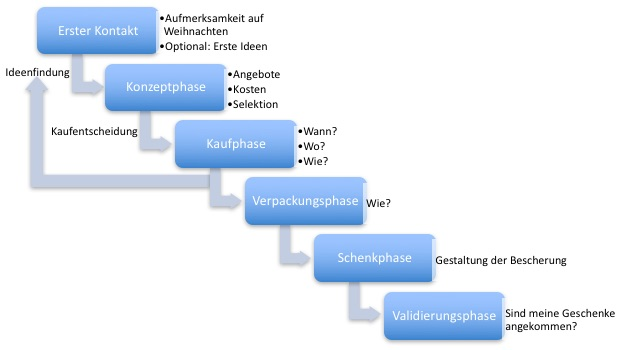
\includegraphics[width=\textwidth]{prozess-schenken}}
    \caption{Verschiedene Phasen des Schenkprozesses (Eigene Darstellung)}
    \label{fig:prozess}
\end{figure}

Durch den Überblick über den Prozess konnten wir nicht nur die Besorgung und die Bescherung als Aspekte des Schenkens zu Weihnachten ausmachen, sondern auch Aspekte wie das Verpacken der Geschenke oder die eigene Zufriedenheit mit der Auswahl. Auf dieser Basis formulierten wir eine allgemeingültige Frage, welche wir zu Beginn des Interviews stellen ohne weitere Anmerkungen zu tätigen, die die befragte Person in bestimmte Richtungen lenken würde. Die Frage lautet:

\paragraph{Wie schenken Sie zu Weihnachten?}
Der Hintergrund genau dieser Frage ist, dass die befragte Person selbst den Aspekt wählt, den sie als erstes mit dem Thema assoziiert. Anschließend ist es für uns möglich mit Warum und Wie fragen den Aspekt auszuleuchten oder bei Stillstand des Gesprächs auf den nächsten Schritt des Prozesses einzugehen. Dafür haben wir folgende Hilfsfragen formuliert:

\begin{itemize}
    \item Wann machen Sie sich zum ersten Mal Gedanken über die Weihnachtsgeschenke?
    \item Woher bekommen Sie Ihre Ideen?
    \item Was beeinflusst Ihre Entscheidung für den Kauf?
    \item Wie kommen Sie an Ihre Geschenke (Wie/Wo)?
    \item Wie und wann verpacken Sie Ihre Geschenke?
    \item Wie läuft die Bescherung bei Ihnen ab?
\end{itemize}

Falls es aus dem Gespräch selbst nicht deutlich wurde, formulierten wir weiterhin Fragen, welche in jedem Interview, ob als Teil des Gesprächs oder als einzelne Frage, gestellt werden sollten:

\begin{itemize}
    \item Wie ist Ihr Verhältnis zu Weihnachten?
    \item Wichtigkeit des Schenkens und des Beschenkt-werdens
    \item Zufriedenheit mit den eigenen Geschenken?
\end{itemize}

Zur Einstufung der interviewten Personen stellten wir weiterhin Fragen zu Alter und Kontaktdaten. Der komplette Fragebogen ist im Anhang \ref{anhang:fragebogen} dargestellt.

\subsection{Örtlichkeit}
Neben der Fragestellung beschäftigten wir uns zudem mit der Örtlichkeit der Befragung. Hier sind wir schnell auf die Idee gekommen, Menschen dort zu befragen wo sie bereits Zeit mitbringen. Haltestellen oder der Karlsruher Hauptbahnhof sind uns direkt als Möglichkeiten eingefallen. Zum einen erfüllt es den Aspekt, dass Menschen dort länger warten und deshalb Zeit mitbringen. Weiterhin gibt es uns auch die Möglichkeit der Observation und damit Zeit, die Befragten besser auszuwählen.

\subsection{Einleitung}
Als letzten Punkt der Agenda für das Treffen haben wir den Begin der Befragung besprochen. Da uns aufgefallen ist, dass viele nur ungern die Wörter Befragung oder Umfrage hören, haben wir eine neue Strategie diesbezüglich entwickelt. Zum einen wollten wir weder das Wort Befragung noch Umfrage erwähnen. Stattdessen entschieden wir, dass wir uns kurz vorstellen und den Hintergrund unserer Befragung nennen. Anschließend sind wir direkt mit unserer Leitfrage gestartet und haben damit den Befragten nicht die Möglichkeit gegeben auszuweichen.

\section{Die zweite Befragung}
Die zweite Befragung fand in der Woche nach der ersten Sitzung statt. Dabei einigten wir uns aufgrund zeitlicher Gründe auf zwei unabhängige Befragungen. Wir wählten wieder die Methode der Befragung, da wir uns erhofften, damit den kompletten Prozess des Schenkens abbilden zu können. Bei der Örtlichkeit einigten wir uns auf den Karlsruher Hauptbahnhof. Wir erwarteten, dass dort viele Passanten unterwegs sein würden, welche gleichzeitig die nötige Zeit mitbringen.

\subsection{Ergebnisse der zweiten Befragung}
\subsubsection{Örtlichkeit}
Der Hauptbahnhof war die ideale Wahl für eine Befragung. Zum einen war es uns möglich die Kandidaten auszusuchen anstatt kurzfristig die Entscheidung zu treffen ob man jemanden befragt, der gerade vorbei läuft. Durch die Übersicht über die Gleise war es leicht möglich einzuschätzen, wie viel Zeit die wartenden Personen mitbringen können.

\subsubsection{Learnings}
Neben der Wahl der Örtlichkeit hat sich die Erarbeitung des Prozesses als auch des Fragebogens als positiv auf die Interviews ausgewirkt. Dabei ging es nicht um die Möglichkeit den Fragebogen abzuarbeiten und damit zum kompletten Prozess Antworten zu besitzen, sondern vor allem darum, Sicherheit in das Gespräch zu bringen und auch Bereiche abzudecken, die nicht offensichtlich durch den Begriff Schenken ins Gedächtnis gerufen werden. Dadurch wurden die Gespräche flüssiger und brachten bessere Ergebnisse zu Tage.

\subsubsection{Key findings der Interviews}
Von der organisatorischen Seite her ist uns aufgefallen, dass Umfragen nur dann positiv von den Interviewten aufgenommen werden, wenn diese keinen störenden Effekt haben. Personen auf der Straße zu interviewen, die momentan andere Dinge zu tun haben, stehen Interview eher negativ gegenüber. Entweder sie lehnen es komplett ab oder sind in ihren Antworten kurz angebunden. Aus diesem Grund sollte man entweder Personen direkt zu Interviews einladen, die somit Zeit dafür mitbringen, oder man interviewt an Orten, an denen die Interviewten die benötigte Zeit mitbringen.\\

Inhaltlich hat das Thema Schenken ein sehr breites Spektrum an Aspekten und wird auf verschiedenste Weisen umgesetzt und angenommen. Jeder der Aspekte kann dabei Probleme auslösen. Hier können vor Allem die Ideenfindung und die Besorgung der Geschenke als größte Probleme angesehen werden. Gleichzeitig treten sowohl absolute Verfechter des Schenkens, als auch Gegner dessen auf. Die Gründe sind dabei ebenso vielfältig: Es gibt religiöse Menschen, welche das christliche Fest in den Vordergrund rücken, als auch Gegner, die entweder das Fest selbst oder den Kommerz hinter dem Schenken ablehnen. Dem gegenüber stehen Personen, für die das Schenken dazu gehört und im Schenken eine Freude für die Beschenkten sehen.

%----------------------------------------------------------------------------------------
%	CHAPTER 2
%----------------------------------------------------------------------------------------
\chapterimage{personas.png}
\chapter{Storytelling}
\setcounter{page}{7}

Der nächste Schritt des Design Thinking beinhaltet das Storytelling. Hierbei geht es um die Wiedergabe der Geschichten der Interviewpartner an die Gruppenmitgliedern und die anschließende Entwicklung von verschiedenen Personae und Point of Views. Dieser Schritt fand vollständig während des Seminartermins am 19. November statt.

\section{Personae}
Aufgrund der Befragung entwickelten wir zuerst zehn verschiedene Personae:

\begin{tasks}(2)
    \task Der subtile Nachfrager
    \task Der Geschenk-Profi
    \task Der persönliche Schenker
    \task Der Pragmatiker
    \task Der Bastler
    \task Der Selber-Macher-Lasser
    \task Der reiche Traumerfüller
    \task Der Religiöse
    \task Der Pflicht-Schenker
    \task Der Grinch
\end{tasks}

Bei der Einteilung der Persona gab es in der Gruppe jedoch deutlich unterschiedliche Einschätzungen. Das lag verstärkt daran, dass es verschiedene Ansichten darüber gab, welche Eigenschaften der Persona relevant sind um die zentrale Motivation zu finden, und welche vernachlässigt werden können. Schlussendlich haben wir uns jedoch auf eine Einteilung geeignet:

\begin{enumerate}
    \item Der Religiöse: Die Persona lehnt schenken an Weihnachten mit dem Hintergrund des christlichen Gedankens ab. Ihr zentrale Motivation an Weihnachten ist das Beisammensein der Familie, das Leben der christlichen Werte und das feiern des Festes im traditionellen, christlichen Sinn.
    
    \item Der Grinch: Diese Persona schenkt an Weihnachten nicht, da sie das Fest selbst nicht feiert. Dies kann dabei zwei Gründe haben. Zum einen sieht die Persona Weihnachten als ein kommerzielles Fest an, was den eigentlichen Hintergrund verloren hat. Zum anderen feiert Sie das Fest nicht, da sie entweder einer anderen oder gar keiner Religion angehört.
    
    \item Der persönliche Schenker, der Geschenk-Profi, der Bastler: In diese Gruppe fallen alle Personae, welche durch ihre hohe Motivation beim Schenken auffallen. Ihre Geschenke sind stets auf den Charakter des Beschenkten zugeschnitten. Anstatt irgendetwas zu schenken, schenken sie lieber gar nichts.

    \item Der Selber-Macher-Lasser: Eine andere Person führt den kompletten Schenkprozess für diese Persona durch. Nur das Schenken selbst wird von der Persona gemacht.
    
    \item Der subtile Nachfrager, der reiche Traumerfüller, der Pragmatiker: Die Personae fragen offen oder verdeckt was die Beschenkten haben möchten. Dabei stehen sie dem Schenken selbst eher pragmatisch gegenüber.
    
    \item Der Pflicht-Schenker: Diese Persona lehnt Weihnachten aus verschiedenen Gründen ab und schenkt nur, weil es entweder eine Tradition ist oder er anderen nicht vor den Kopf stoßen möchte.\\
\end{enumerate}

Weiterhin lassen sich diese Gruppen noch grob danach ordnen, wie sie sowohl Weihnachten als auch dem Schenken gegenüber stehen. Diese Einordnung stellt dabei besser da, auf welcher Ebene des Schenkens die Needs der Persona sind: ob sie schon das Schenken selbst ablehnen oder am Geschenkprozess etwas ändern möchten.

\begin{figure}[ht]
    \centering
      \makebox[\textwidth]{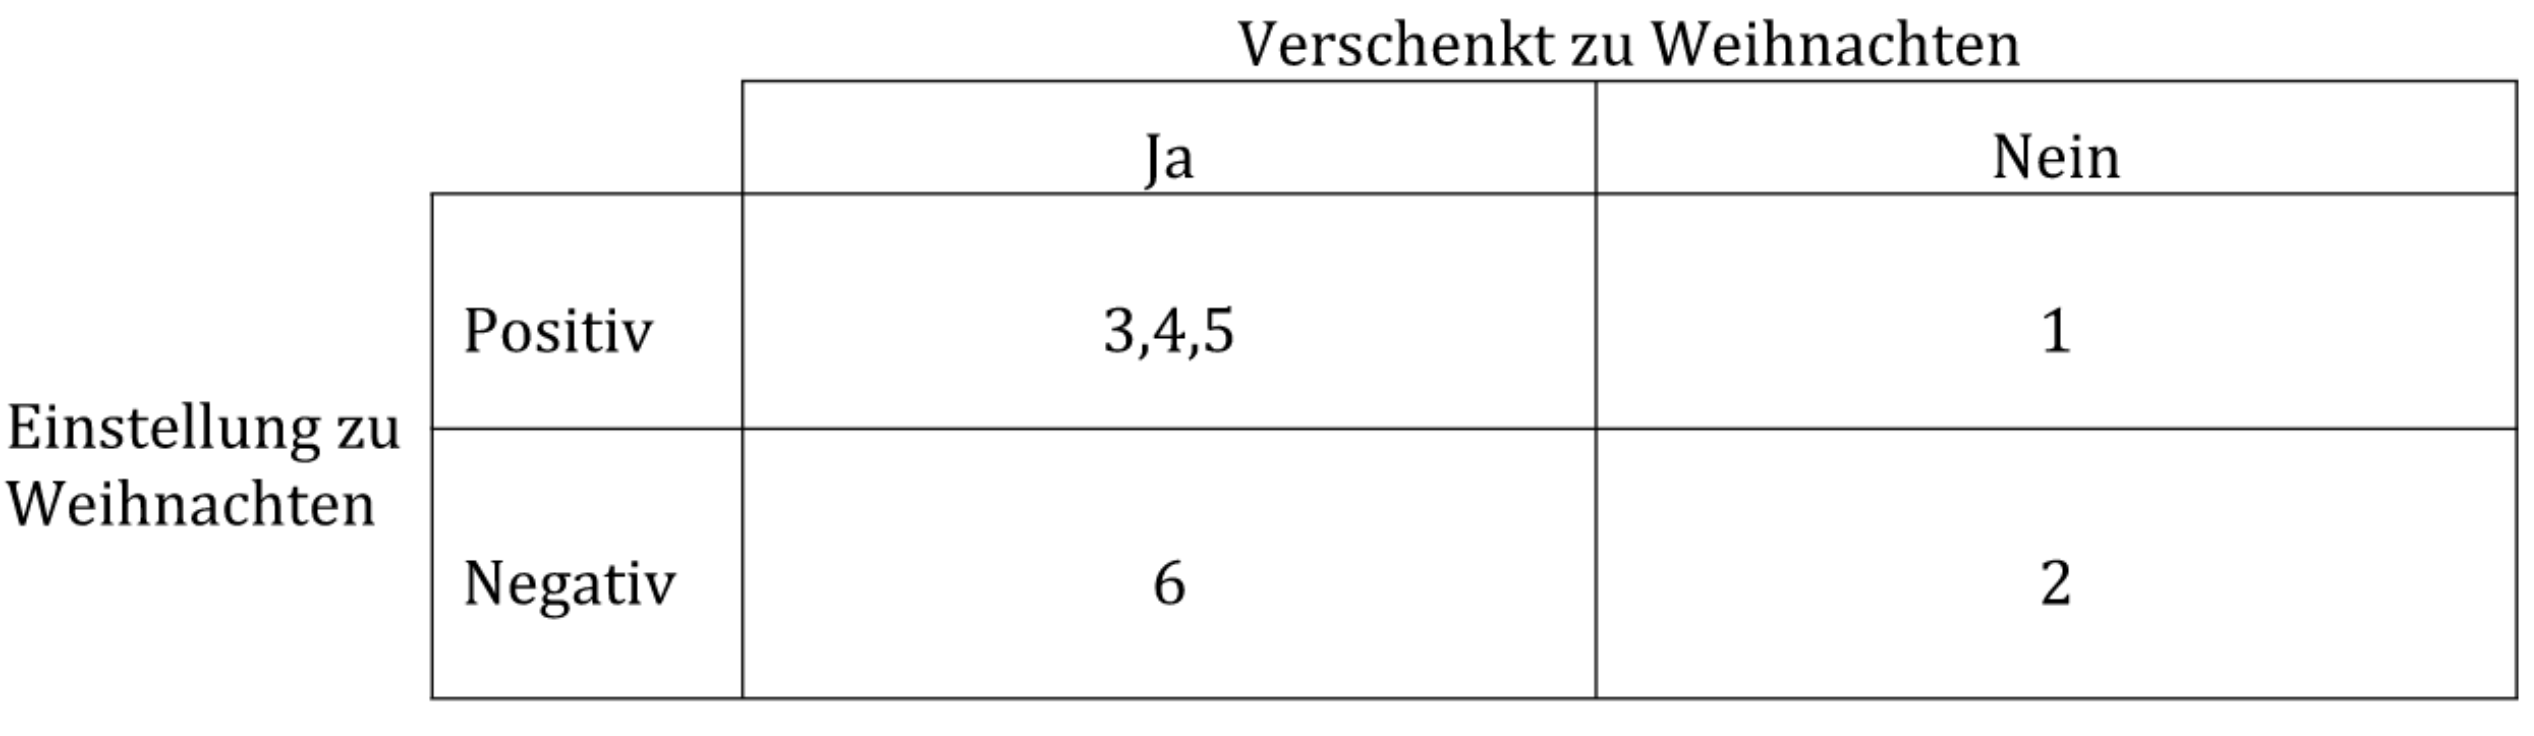
\includegraphics[width=\textwidth]{positiv}}
    \caption{Einordnung der Gruppen}
    \label{fig:positiv}
\end{figure}

\section{Detaillierte Personae}
Aus diesen sechs Personae beschrieben wir drei detaillierter. Zwei davon befinden sich im Anhang \ref{anhang:Personae}. Dabei wollten wir vor allem die Insights und Needs herausspiegeln, auf die wir später die Point of View aufbauen wollen.

\subsection{Der Pflicht-Schenker}
\textbf{Name & Alter:} Peter Ohlenschläger, 31\\
\textbf{Familien- und sozialer Status:} Ledig\\
\textbf{Stadt:} Karlsruhe\\
\textbf{Beruf & Einkommen:} Wissenschaftlicher Mitarbeiter (Doktorand) am KIT, Bereich Theoretische Physik\\
\hline
\paragraph{Rolle & Position im Stakeholder-Netzwerk:}
Peter ist Single und lebt in einer 3er WG in der Karlsruhe Oststadt. Nach seinem Studium der Physik hat er am Lehrstuhl für Physik angefangen seine Doktorarbeit zu schreiben. Er versteht sich gut mit seinen Kollegen, mit denen er jeden Tag zu Mittag isst und als einen seiner Freundeskreise ansieht. Neben diesem engagiert er sich trotz Doktorstelle weiterhin im Arbeitskreis Kunst und Kultur (AKK), das er bereits seit seinem ersten Semester tut. Sven ist kein Familienmensch. Da diese weiterhin im Dorf leben fühlt er sich ihnen gegenüber fremd, da er sich weiterentwickelt hat, während sie das nicht getan haben. Aus diesem Grund besucht er die Familie unregelmäßig, häufig nur an den großen Feiern (Geburtstag, Weihnachten, ...). Zu seinen zwei Schwestern hat er hierbei jedoch noch das beste Verhältnis.\\
\hline
\paragraph{Hobbies & Identifizierungsmaßnahmen:}
Peter liebt Knobelspiele. Aus dieser Liebe hat sich später auch das Interesse an Mathematik und Physik entwickelt. Er geht gerne auf Konzerte und Festivals, vor allem in die Richtung Hard Rock/Metal. Bandshirts, lange Haare und sein Bart sieht er als seine Erkennungszeichen an. Wenn er nicht gerade auf Konzerten anzutreffen ist, tümmelt er sich entweder am AKK oder in den verschiedenen Bars, bevorzugt Irish Pubs, Karlsruhes herum. Da er dieses Hobby bereits in seiner Kindheit hatte, spielt er jetzt noch regelmäßig Computerspiele. Inzwischen zwar deutlich reduziert, setzt er sich 1-2 mal pro Woche noch vor seinen Computer.\\
\hline
\paragraph{Pain Points & Needs / Einstellung gegenüber ... (brand, service, problem, topic):}
Obwohl Peter kein inniges Verhältnis zu seiner Familie hat, hat er nicht das dringende Bedürfnis dieses Verhältnis zu verbessern. Er hat in den Freunden und Kollegen in Karlsruhe genug sozialen Halt gefunden. Natürlich interessiert ihn weiterhin die Familie, dieses Interesse basiert jedoch auf eine Art innere Pflicht die er verspürt. Wenn er in  seiner Heimat ist, ist er schnell gelangweilt und des Öfteren genervt von den Fragen und Einstellungen seiner Eltern und Geschwister.
Diese Einstellung gegenüber seiner Familie ist ein zentraler Aspekt wenn es darum geht, dass er zu Weihnachten nach Hause geht. Am liebsten würde er einfach in Karlsruhe bleiben und die Feiertage mit Freunden verbringen oder komplett seine Ruhe haben. Weihnachten steht er aber auch in anderer Ansicht negativ gegenüber: Er mag den kommerziellen Aspekt des Festes nicht. Diese gezwungene Schenken findet er sehr nervig und steht dem sehr kritisch gegenüber. Aufgrund der Distanz zu seiner Familie fällt es ihm sehr schwer, die richtigen Geschenke zu finden. Daraus folgt oft, dass er irgendetwas schenkt. Trotz dieser Ansichten gegenüber seiner Familie und Weihnachten hat er das Bedürfnis, den Familiensegen aufrecht zu erhalten. Deshalb nimmt er trotz seiner Ablehnung jedes Jahr an Weihnachten teil und beschenkt seine Familie.\\
\hline
\paragraph{Ziele & Träume:}
Peters berufliches Ziel ist es eine wissenschaftliche Karriere zu haben. Er kann sich gut vorstellen, zukünftig als Professor zu lehren. Im gefallen die Offenheit, Neugierde und der Freigeist der Universität und der Forschung.\\
\hline
\textbf{Drei Dinge, ohne die er nicht Leben kann:} Musik, das AKK und seine Freunde \\
\textbf{Ich bin gut in:} Mathematik und logisches Verständnis, Zocken,  ehrenamtliches Engagement \\
\textbf{Ich wünschte ich wäre gut in:} Schlagzeug spielen (wäre gerne Mitglied einer Band) \\
\textbf{Mein nächstes großes Event wird:} Verteidigung der Dissertation \\
\textbf{Mein Traumurlaub war:} Die jährliche Fahrt auf das Wacken \\
\textbf{In meinem Kühlschrank ist immer:} Bier \\
\hline

%----------------------------------------------------------------------------------------
%	KAPITEL 3
%----------------------------------------------------------------------------------------
\chapterimage{ideation.png}
\chapter{Ideation}
\setcounter{page}{11}

Nachdem die Personae entwickelt wurden, geht es in der Ideation darum, das zentrale Bedrüfnis der Persona zu finden und auf der Grundlage dieses Lösungsansätze zu finden. Hier wird zuerst ein Point-of-View entwickelt und eine Base of Ideation kreiert. Schlussendlich findet die Ideenfindungen statt, welche in der Herausarbeitung einer konkreten Idee endet.\\

\section{Der Point-of-View von Peter Ohlenschläger}
Wir haben uns Gedanken gemacht, welche Persona am offensichtlichsten einen Need besitzt, der gleichzeitig einfach zu lösen ist. Dafür haben wir das zentrale Bedürfnis der Persona herausgesucht und analysiert:

\begin{itemize}
    \item \textbf{Der Pragmatiker:} Ihm ist die Familie wichtig, weshalb er versucht das richtige Geschenk für die Person zu finden. Dabei befragt er die Personen indirekt, z.B. über Geschenklisten an den Weihnachtsmann, oder direkt. Seine größte Problematik ist die geringe Zeit, die er besitzt um die Geschenke zu besorgen.
    \item \textbf{Der Grinch:} Durch das abgekühlte Verhältnis zu seiner Familie hat er bereits vor Jahren bereits aufgehört Weihnachten zu feiern. Er hat darüber hinaus eine negative Einstellung zu Weihnachten entwickelt.
    \item \textbf{Der Pflicht-Schenker:} Diese Persona hat eine negative Einstellung gegenüber Weihnachten, fühlt jedoch einen sozialen Druck gegenüber seiner Familie, an Weihnachten und dem Schenken teilzunehmen.\\\\
\end{itemize}
Es fällt sofort auf, dass der Grinch ein grundsätzliches Problem mit Weihnachten besitzt und sein Need nicht durch einen einfachen Service oder Gut zu lösen ist. Wir haben uns aus diesem Grund gegen ihn entschieden. Dem Pragmatiker fehlt wiederum nur Zeit. Da er seine Ideen bereits besitzt haben wir uns gegen ihn entschieden. Es gibt bereits zu viele Services, die diese Problematik lösen können.

Schlussendlich haben wir uns für den Pflicht-Schenker entschieden. Hier sehen wir das Potential, dass man ihm durch einen einfach Service das Geschenke-Finden und –Kaufen deutlich vereinfachen kann.

\begin{figure}[ht]
    \centering
      \makebox[\textwidth]{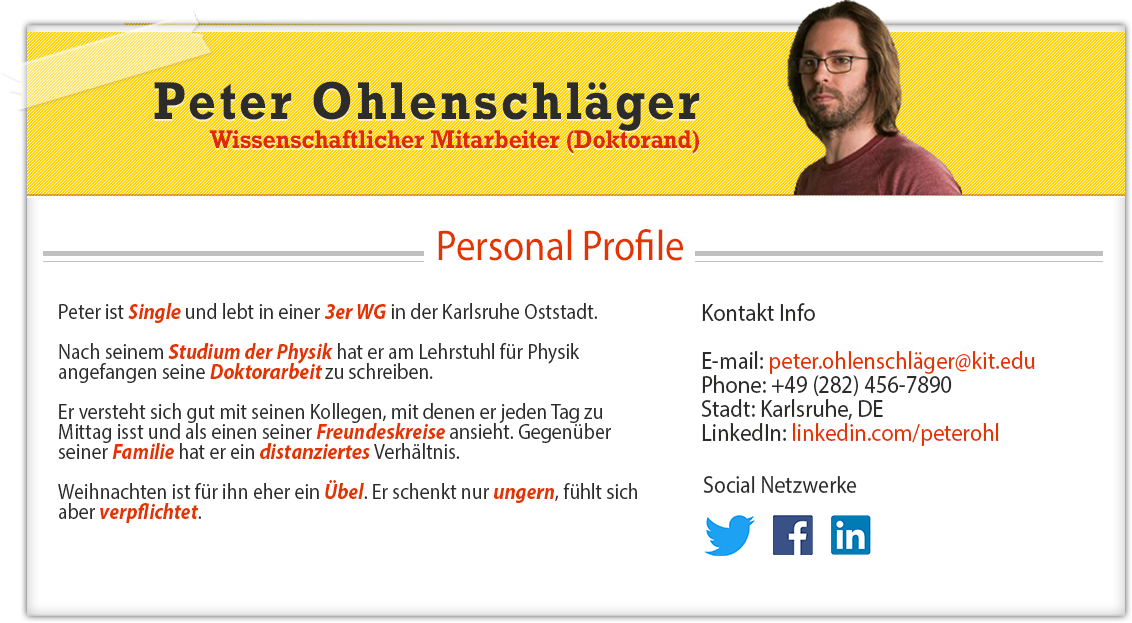
\includegraphics[width=0.9\textwidth]{peter2}}
    \caption{Der Pflichtschenker Peter Ohlenschläger (eigene Darstellung)}
    \label{fig:peter}
\end{figure}

\section{Base of Ideation}
Für Peter den Pflicht-Schenker entwickelten wir eine Base of Ideation, also eine Fragestellung anhand der wir den Need in die verschiedenen Aspekte aufteilen können. Die zentrale Fragestellung ist dabei:

\paragraph{How might we help Peter to find inspiration?}

Daraus resultieren die Splitterfragen:
\begin{itemize}
    \item How to find ideas?
    \item How to get the presents?
    \item How to reduce the effort?
\end{itemize}

\section{The 5 ideas}
Als nächsten Schritt machten wir uns daran, mögliche Lösungsansätze aus diesen Splitterfragen zu generieren. Dabei dachte jeder für sich selbst nach und sammelte Vorschläge, welche anschließend mit der ganzen Gruppe besprochen und ähnliche gruppiert wurden. Aus dieser Wolke an Ideen suchte jedes Gruppenmitglied eine Idee aus. Es wurden folgende fünf Ideen gewählt:

\begin{itemize}
    \item Eine Geschenkplattform, die das Geschenke-Finden und –Einkaufen vereinfacht
    \item Eine geführte Erlebniseinkaufstour, welche das Geschenke-Finden und –Einkaufen mit Spaß verbindet (z.B. anschließende Kneipentour, Sportevents, etc.)
    \item Ein Reiseservice, der einen Fluchtort vor Weihnachten anbietet (z.B. Weihnachten auf einer Insel)
    \item Ein Wellnesscenter mit Geschenkeservice. Hier soll neben dem Wellnessprogramm die Vorführung verschiedener Geschenkideen stattfinden
    \item Ein Weihnachtseinkaufscenter, indem die verschiedenen Geschenkkategorien in einzelne Läden aufgeteilt sind und durch individuellen Service der Kunde einfach und schnell Geschenke finden und kaufen kann.\\
\end{itemize}

Diese Ideen wurden anschließend von jedem Einzelnen noch erweitert. Dabei überlegte sich jeder kurz wie er die Idee weiter ausschmücken würde. Die vollständig erweiterten Ideen sind im Anhang \ref{anhang:ideen} zu finden.

Diese fünf ausgearbeiteten Ideen wurden auf Ihre Feasibility, Desirability und Viability untersucht. Dabei sind wir auf das Ergebnis gekommen, dass die Geschenkeplattform insgesamt am besten abschneidet. Aus diesem Grund haben wir diese Idee gewählt.

\begin{table}[ht]
\begin{center}
\begin{tabular}{l*{3}{c}r}
Idee & Desirability & Feasibility & Viability & Gesamt\\
\hline
Geschenkplattform & 3  & 3 & 1 & 7\\
Geführte Erlebnis-Einkaufstour & 2  & 2 & 2 & 6 \\
Weihnachten auf einer Insel & 2  & 1 & 3 & 6\\
Wellnesszentrum mit Geschenkservice & 2 & 1 & 2,5 & 5,5\\
Weihnachts-Einkaufzentrum & 1,5 & 1 & 1 & 3,5\\
\hline
\end{tabular}
\end{center}
\caption{Einschätzung der Gruppen zu Feasability, Desirability und Viability (Eigene Darstellung)}
\label{tab:feasability}
\end{table}%

%----------------------------------------------------------------------------------------
%	CHAPTER 4
%----------------------------------------------------------------------------------------

\chapterimage{protyping.png} % Chapter heading image
\chapter{Prototyping}
\setcounter{page}{14}
%\begin{figure}[ht]
 %   \centering
  %    \makebox[\textwidth]{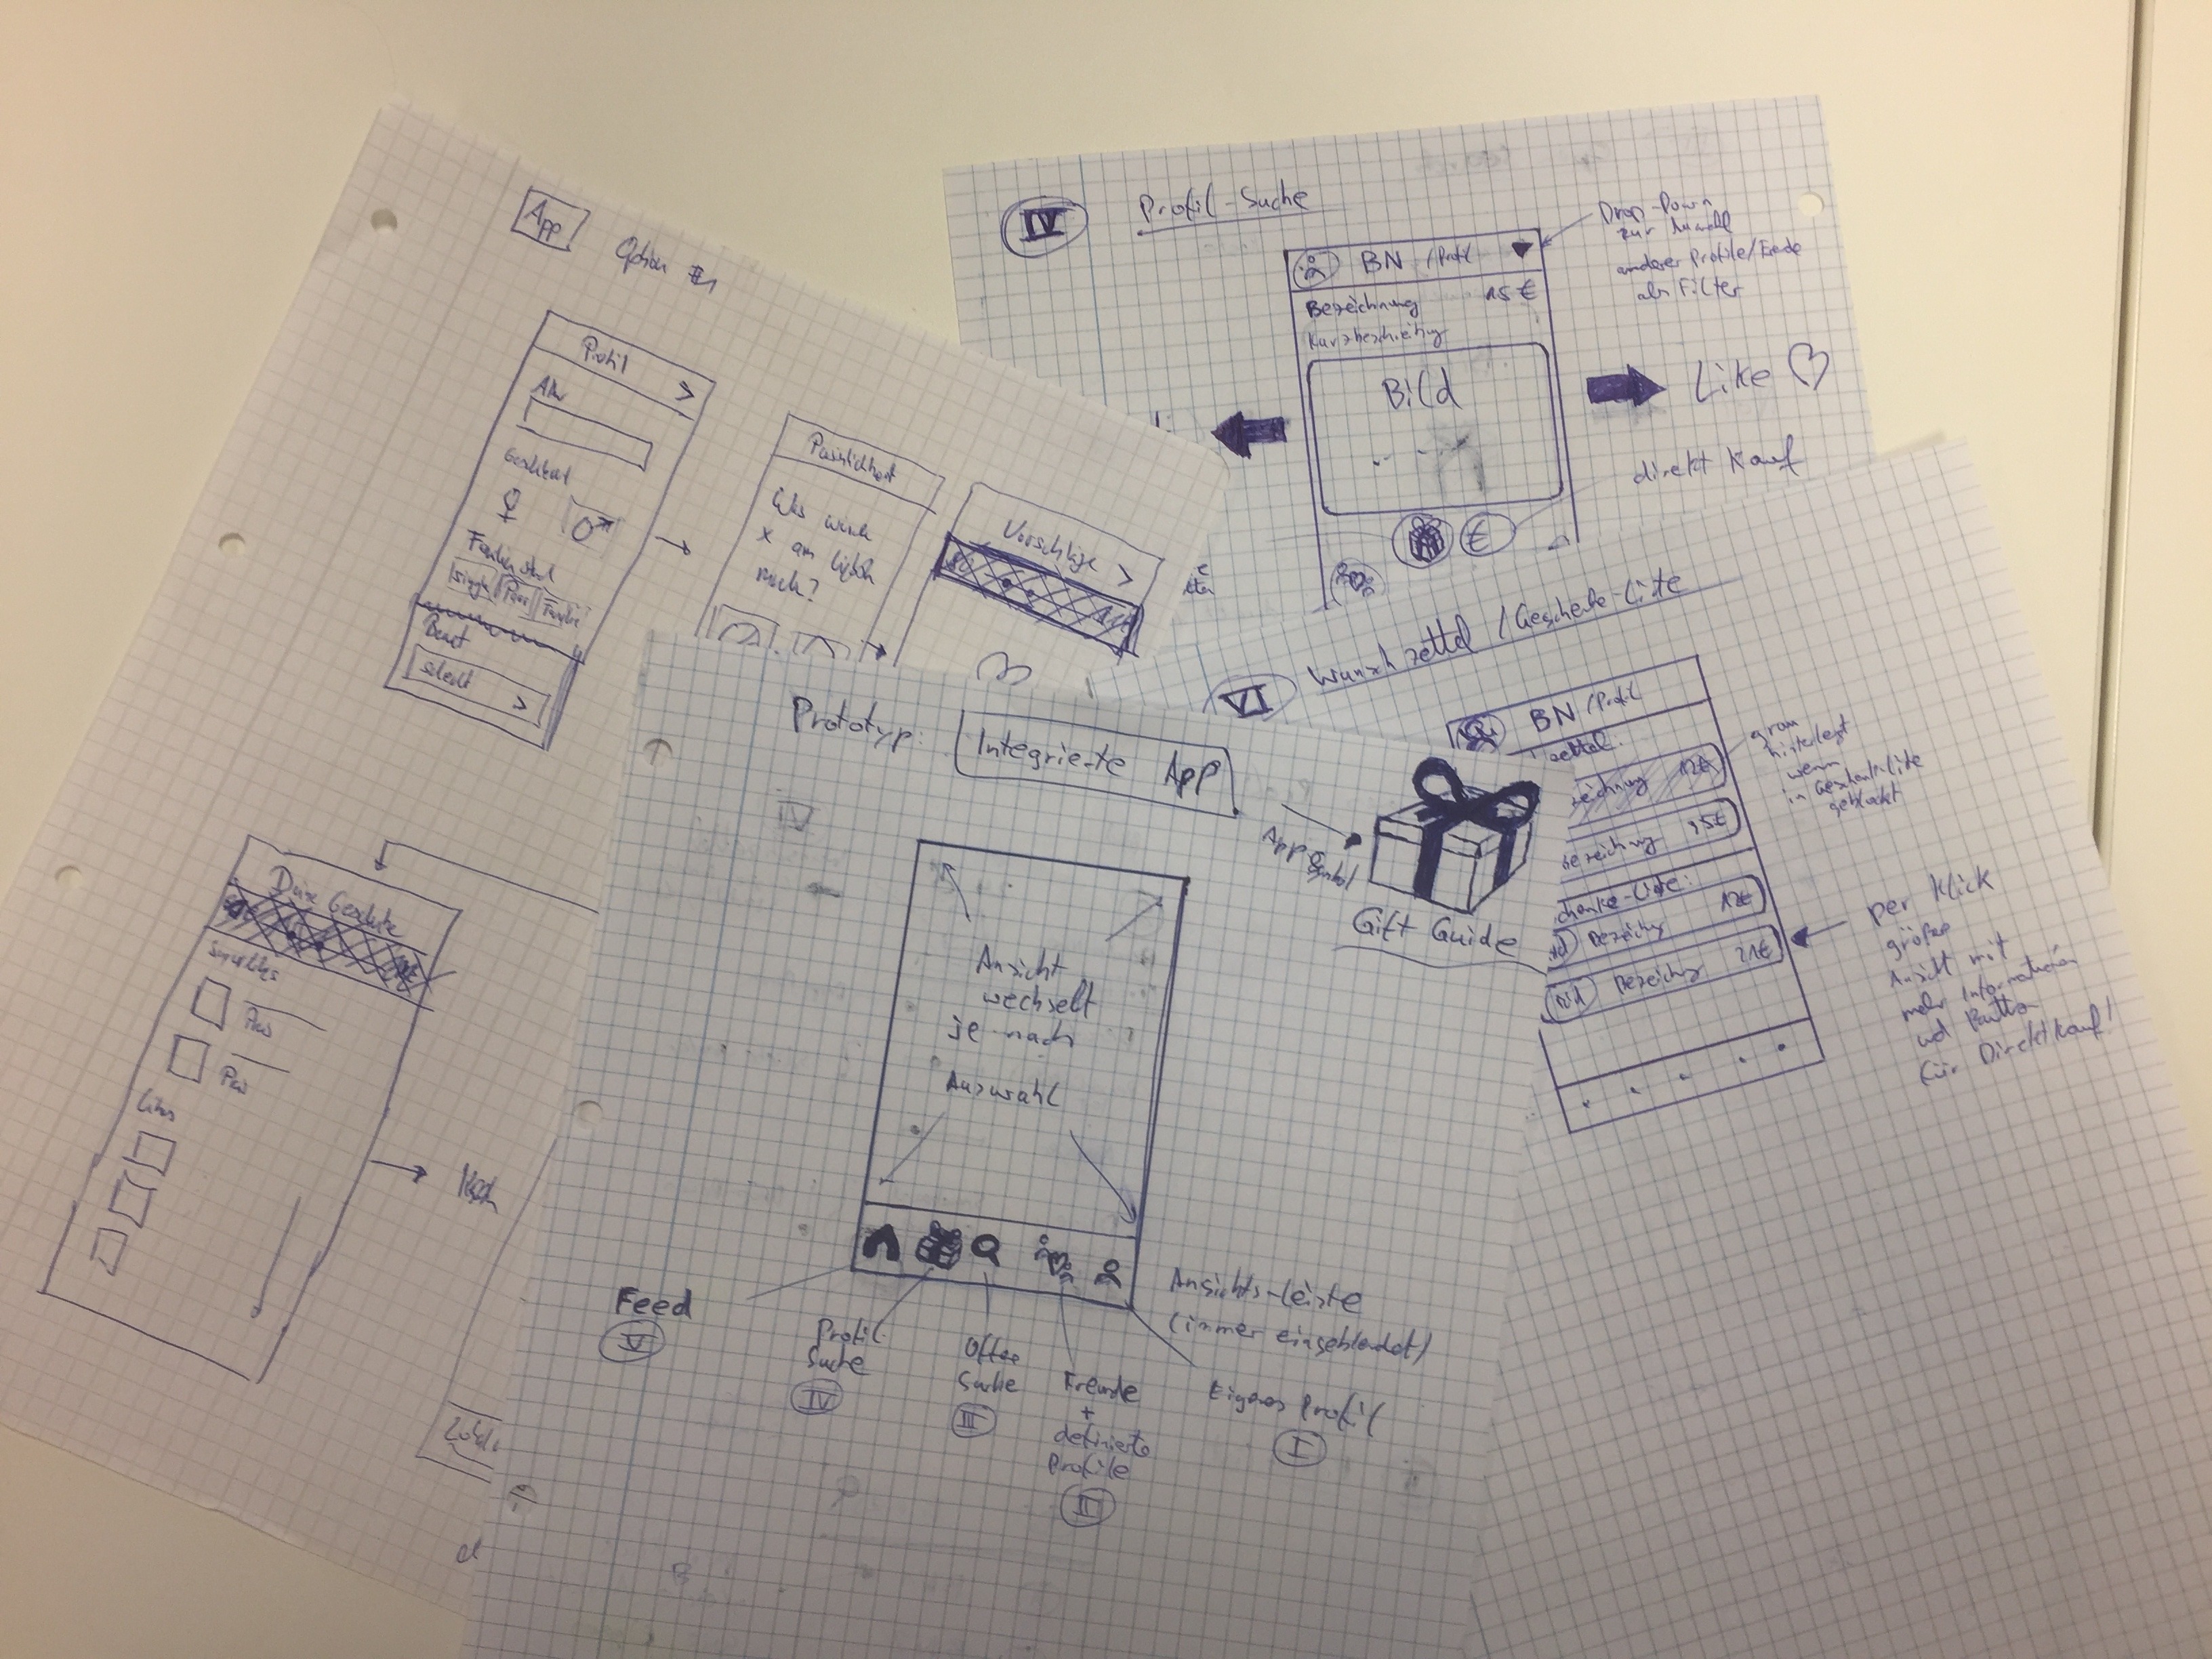
\includegraphics[width=0.75\textwidth]{ptoto_0}}
   % \caption{"Hand-made" Prototypes (Version 0.1)}
  %  \label{fig:peter}
%\end{figure}

Nach Auswahl der groben Produktidee ging es an die konkrete Ausgestaltung in Prototypen. In einer ausführlichen Diskussionsrunde zeigte sich, dass die einzelnen Teammitglieder doch sehr unterschiedliche Vorstellungen von dem Endprodukt hatten. Um die Variantenvielfalt zu beherrschen, versuchten wir eine Art „Morphologischen Kasten“ zu bauen, in dem jeder Eigenschaft des Prototypen die möglichen Ausprägungen zugeordnet werden und die Auswahl einer Ausprägung aus jeder Eigenschaft eine Variante ergibt. Es zeigte sich, dass die Varianten aufgrund von gegenseitigen Abhängigkeiten und Ausschlusskriterien, doch besser in einer Art Prozessablauf dargestellt werden konnten, wobei den einzelnen Prozessschritten jeweils mehrere Ausprägungen zugeordnet wurden.\\

Nach der Abbildung der Gesamtkomplexität des Entwicklungsproblems wurde in einer „Rapid-Prototyping-Runde“ von jedem einzelnen Teammitglied in wenigen Minuten die Grobskizzierung eines Prototypen nach den eigenen Vorstellungen als „Version 0.1“ durchgeführt. Die entstandenen, eher groben, Prototypen wurden gemeinsam weiter ausgestaltet und modifiziert, um einen möglichst großen Bereich der Kombinationsmöglichkeiten abzudecken und mit offenen Augen die Reaktionen der Endnutzer im Protypen-Test beobachten zu können, ohne Ausprägungen von vorneherein auszuschließen. Die Ergebnisse wurden digital in „Balsamiq Mockups 3“ umgesetzt.

\begin{figure}[ht]
    \centering
      \makebox[\textwidth]{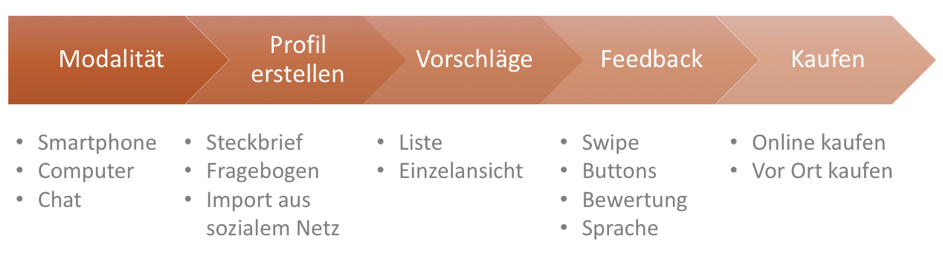
\includegraphics[width=\textwidth]{geschenkplattform}}
    \caption{Prozessablauf der Geschenkplattform}
    \label{fig:peter}
\end{figure}

Die dabei entstandenen Test-Prototypen werden im Folgenden vorgestellt. Eine Großansicht der einzelnen Prototypen befindet sich im Anhang. 

\section{Test-Prototypen (Version 1.0)}
Da alle Prototypen auf dem gleichen Prozessablauf basieren, weisen diese auch die gleiche Struktur in ihrer Grundfunktion auf. Grundsätzlich wird in der jeweiligen Modalität ein Profil des zu Beschenkenden definiert. Auf Basis dieses Profils werden passende Geschenkvorschläge gemacht, welche durch ein Feedback bewertet werden können. Am Ende des Prozesses können die ausgewählten Produkte näher betrachtet und entweder online gekauft werden oder es werden lokale Kaufmöglichkeiten angezeigt.

\subsection{Swipe-App (Prototyp 1)}
\begin{figure}[ht]
    \centering
      \makebox[\textwidth]{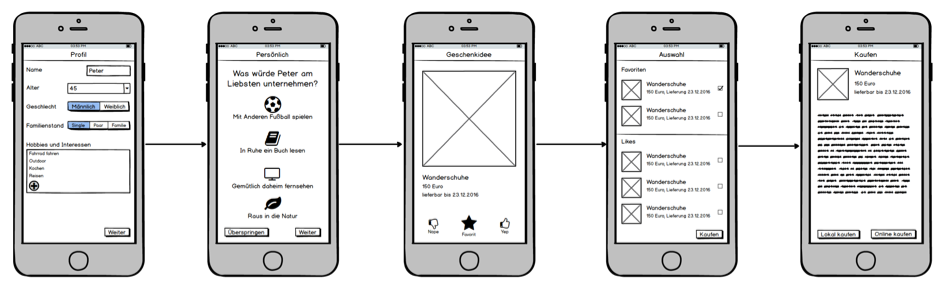
\includegraphics[width=\textwidth]{swipe-app}}
    \caption{Swipe-App (Prototyp 1)}
    \label{fig:proto1}
\end{figure}

Bei der Swipe-App wird das Profil zunächst durch einen Steckbrief definiert, wobei spezielle Tags für Hobbies und Interessen ergänzt werden können. Anschließend wird das Profil durch „What if“-Persönlichkeitsfragen ergänzt, um das Profil weiter zu detaillieren. Die anschließenden Geschenkvorschläge können durch Swipen mit „Nope“ oder „Yep“ bewertet oder als „Favorit“ markiert werden, wobei die Ergebnisse in entsprechenden Listen abgespeichert werden. Aus den Listen kann das favorisierte Geschenk ausgewählt und in der Detailsicht letztendlich online oder vor Ort gekauft werden. Dieser Prototyp besticht gerade durch seine Einfachheit. 

\subsection{Chat-Bot (Prototyp 2)}
\begin{figure}[ht]
    \centering
      \makebox[\textwidth]{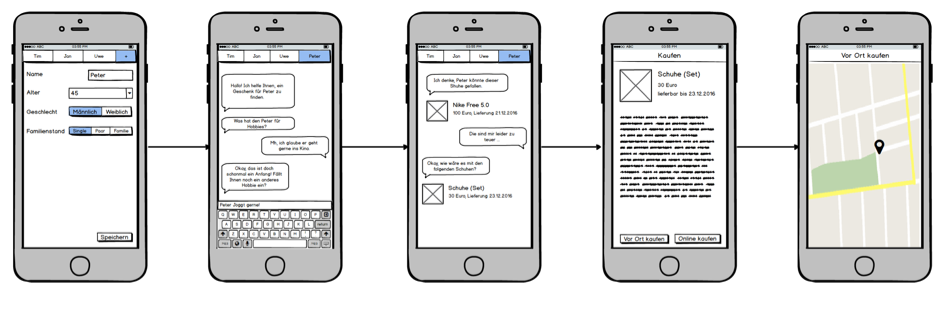
\includegraphics[width=\textwidth]{bot}}
    \caption{Chat-Bot (Prototyp 2)}
    \label{fig:proto2}
\end{figure}

Bei dem Chat-Bot wird zunächst analog das Profil durch einen Steckbrief erstellt. Im Unterschied ist jedoch die Grundidee, die weitere Detaillierung des Profil, sowie die Generierung der Geschenkvorschläge und deren Bewertung im Dialogstil durchzuführen. Es werden also weitere Fragen zur Person gestellt und dazu Geschenkvorschläge gemacht. Je nach Eingabe des Feedbacks werden dann weitere detaillierende Fragen gestellt und neue Vorschläge generiert. Der Vorteil liegt hierbei in der ausführlicheren Form des Feedbacks, wobei nicht nur ein Ja- oder Nein-Feedback gegeben werden kann, sondern zusätzlich Begründungen, welche die weiteren Vorschläge verbessern können. Aufgrund der schweren Programmierbarkeit des Bots, könnte ein Ansatz auch auf realen Service-Mitarbeitern basieren.

\subsection{Webseite (Prototyp 3)}
\begin{figure}[ht]
    \centering
      \makebox[\textwidth]{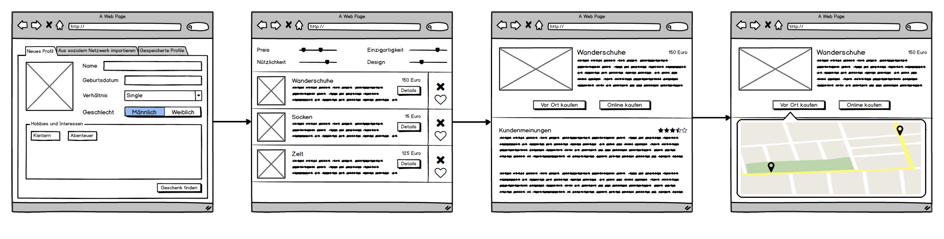
\includegraphics[width=\textwidth]{website}}
    \caption{Webseite (Prototyp 3)}
    \label{fig:proto3}
\end{figure}

Die Webseite findet am Computer statt und befindet sich damit in einer anderen Modalität. Zusätzlich können Profile aus sozialen Medien importiert werden. Ein weiterer Vorteil besteht in der Detaillierung der Attribute des Geschenkes durch Schieberegler je nach Preis, Design, Nützlichkeit oder Einzigartigkeit. Gerade der Preis scheint ein notwendiger Filter zu sein, um zu teure oder zu günstige Geschenke auszuschließen. Im Gegensatz zur Smartphone Applikation und dem Chat-Bot, werden die Vorschläge in Listenform angezeigt. Werden in dieser Liste Vorschläge durch „X“ entfernt, rücken die unteren Vorschläge nach Oben. Positiv bewertete Vorschläge rücken an den Anfang der Liste. Durch den Button „Details“ können ebenfalls weitere Informationen eingesehen werden und die Kaufoptionen ausgewählt werden. 

\subsection{Soziales Netz (Prototyp 4)}
\begin{figure}[ht]
    \centering
      \makebox[\textwidth]{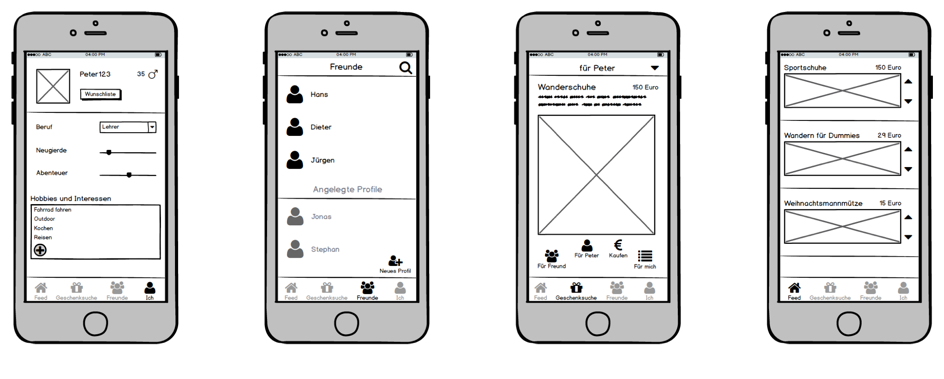
\includegraphics[width=\textwidth]{social}}
    \caption{Soziales Netz (Prototyp 4)}
    \label{fig:proto4}
\end{figure}

Das soziale Netz stellt eine Art erweiterte Form der Swipe-App (Prototyp 1) dar. Neben der Definition der Profile der Beschenkten, kann auch ein Profil des Nutzers selbst erstellt werden. Dadurch können Nutzer eine Freundesliste aufbauen und auch mit den selbst erstellten Profilen ihrer Freunde nach passenden Geschenken für diese suchen. Alternativ können sie auch mit ihrem eigenen Profil nach Produkten suchen, die ihnen gefallen könnten. Neben der Geschenkesuche, kann die App also auch als ganzjährige Shopping-App genutzt werden. Eine weitere Zusatzfunktion bietet der Wunschzettel, den jede Person für sich selbst definieren kann und der wie eine „American Wedding List“ funktioniert. Freunde können diese Wunschliste einsehen und dort Geschenke auswählen und diese für die weiteren Freunde blockieren, ohne dass der Nutzer dies sieht. Damit können Wünsche geäußert werden ohne offen darüber zu sprechen und gleichzeitig Doppelkäufe von Geschenken vermieden.\\

Per Swipe können die Vorschläge vor- und zurückgeschaltet werden. Der Auswahl-Mechanismus findet durch Anklicken des jeweiligen Profils statt, wobei der Vorschlag für jedes Profil gespeichert werden kann. Die am häufigsten ausgewählten Vorschläge werden im Feed angezeigt und von der Community up- und down-gevotet. So können im Feed die beliebtesten Geschenke über alle Profile in der Community eingesehen werden. Am unteren Bildrand kann analog zu aktuellen Apps jederzeit zwischen dem eigenen Profil, der Freundesliste, der Geschenksuche und dem Feed gewechselt werden. 

%----------------------------------------------------------------------------------------
%	CHAPTER 5
%----------------------------------------------------------------------------------------
\chapterimage{testing.png} % Chapter heading image
\chapter{Testing}
\setcounter{page}{18}

Abschließend zur Entwicklung der Prototypen wurde diese im Rahmen einer weiteren Befragung mit 23 Personen getestet. Dabei wurden die Prototypen in ausgedruckter Form den Probanden vorgelegt und die Funktion dieser mit den Probanden durchgespielt. Sowohl während der Benutzung, als auch am Ende wurde Feedback vom Benutzer eingeholt, wobei wir uns während der Benutzung auf Anregungen des Nutzers fokussiert haben. Alle Probanden spielten alle Prototypen durch. \\

\section{Auswertung der Befragungen}

Im Vergleich der Prototypen kamen sowohl die Swipe-App (Prototype 1) als auch die Webseite (Prototyp 3) am besten an. Der Chatbot (Prototype 2) und das soziale Netz (Prototyp 4) hingegen wurden eher skeptisch bewertet. Bei den Befragungen konnten starke Unterschiede innerhalb der Zielgruppe festgestellt werden. So wurde eine Smartphone-App mit Detailansicht und Swipe-Funktion von den jüngeren Probanden (Anfang 30) besser angenommen, die älteren Personen unserer Zielgruppe (Ende 40) waren eher gegenüber einer Webseite mit Listenansicht aufgeschlossen. Überraschend für uns war, dass ein Angebot zum lokalen Kaufen sehr beliebt war. Diese Funktion wurde durchgehend gelobt.

\section{Quantitative Bewertung der Prototypen}

Eine quantitative Bewertung der Prototypen haben wir in Tabelle \ref{tab:quantitative_bewertung_prototyp} vorgenommen. Klar zu sehen ist, dass die Webseite am beliebtesten unter den Prototypen ist, während der Chatbot (Prototyp 2) und das soziale Netz (Prototyp 3) nicht so gut angenommen wurden. Gleichzeitig sind diese Prototypen ebenfalls am schwersten umzusetzen. Für den Chatbot muss ein maschinelles Lernverfahren eingesetzt werden, welches mit geschriebener Sprache umgehen kann, um eine natürliche Interaktion zu ermöglichen. Für die Realisation eines sozialen Netzes wird eine kritische Masse an Benutzern benötigt, damit das Produkt funktioniert. Gerade zu Beginn stellt dies eine große Herausforderung dar. Allen Prototypen gemein ist, dass sie Zugriff auf eine Datenbasis an Geschenkinformationen haben müssen. Die Rentabilität der Prototypen ist bei allen gleich und als eher niedrig einzustufen. Abhängig vom Geschäftsmodell können beispielsweise durch Werbeinnahmen, Partnerprogramme oder einen kostenpflichtigen Zugang Einnahmen generiert werden.

\begin{table}[ht]
\begin{center}
\begin{tabular}{l*{3}{c}r}
Prototyp & Desirability & Feasibility & Viability & Gesamt\\
\hline
Swipe-App (Prototyp 1) & 2 & 3 & 1 & 6\\
Chatbot (Prototyp 2) & 1 & 1 & 1 & 3 \\
\textbf{Webseite (Prototyp 3)} & \textbf{3}  & \textbf{3} & \textbf{1} & \textbf{7}\\
Soziales Netz (Prototyp 4) & 1 & 1 & 1 & 3\\
\hline
\end{tabular}
\end{center}
\caption{Quantitative Bewertung der Prototypen zu Feasability, Desirability und Viability (Eigene Darstellung)}
\label{tab:quantitative_bewertung_prototyp}
\end{table}%

\section{Zusammenfassung des Testens}
Ein grundsätzliches Interesse an der Lösung des Problems sowie an unseren Ideen konnte festgestellt werden. Die Webseite hat sich als stärkster Prototyp hervorgetan. Sie bietet sich als altersunabhängige Lösung in unserer Zielgruppe an. Ebenso gab es nur wenige Kritikpunkte zu diesem Prototyp. Um diese näher erforschen zu können, wird ein vollfunktionaler Prototyp benötigt. Es handelte sich bei den genannten Punkten um Aspekte die Formulierungen (Bsp.: „Alter“ statt „Geburtsdatum“) sowie die Qualität der Vorschläge betrafen. Letztere zeigten sich als essentiell für den Markterfolg.

\section{Weitere Schritte der Umsetzung}
Für die weiteren Schritte müsste der Prototyp zu einer funktionalen Webapplikation ausgebaut werden. Parallel dazu müsste eine Basis an Geschäften und Märkten aufgebaut werden, die die Grundlage für die Geschenkvorschläge bildet. Hinzu kommt, dass gezielt Werbung für den Service geschaltet werden müsste, um die Applikation bekannt zu machen. Testweise kann der erste Release in Karlsruhe stattfinden. Dadurch wäre der Aufwand der ersten Schaffung der Basis sowie der Werbung nicht zu groß. Hier könnte die Applikation weiterhin an der breiten Masse getestet werden. Falls diese Tests positiv ausfallen sollten, wäre eine geografische Ausbreitung denkbar.


\chapterimage{schluss.png} % Chapter heading image
\chapter{Schluss} \\
\setcounter{page}{20}

Design Thinking ist ein nützliches Instrument zur Ideengenerierung. Durch die intensive Befragung und Beobachtung der Zielgruppe können Problemstellungen ermittelt, welche nicht offensichtlich an den Tag treten. Das Problem hierbei ist jedoch, dass durch die intensive Auseinandersetzung mit dem Anwender viel Zeit und Mittel verschlungen werden können. Diese Problematik erweitert sich dadurch, dass die Möglichkeit, zu vorangehende Schritte wieder zurückzukehren, besteht.\\
Aufgrund des geringen zeitlichen Rahmens des Seminars war uns diese Freiheit nicht jedoch gestattet. Gerade die Auseinandersetzung mit dem Anwender beim Interview und beim Testen musste von uns zeitlich beschnitten werden um das Seminar rechtzeitig umsetzen zu können. Besonders diese Freiheit wird von uns jedoch als zentral erachtet, denn erst dadurch ist es möglich, ohne konkretes Streben nach einer Lösung arbeiten zu können. So merkten wir, dass wir oftmals vorschnell an konkreten Lösungsansätzen arbeiteten obwohl der Prozessschritt das nicht vorsah.\\
Uns ist weiterhin aufgefallen, dass die Spannweite des Alters unserer Zielgruppe deutlich zu groß war. Diese Problematik kristalisierte sich noch nicht bei den ersten Befragungen heraus. Hier entstand eine Persona, welche alle Altersgruppen abbilden konnte. Die Lösung, welche wir für diese Persona entwickelten, war jedoch schlussendlich für viele ältere Anwender weniger attraktiv. Hier ist uns jedoch auch bewusst, dass durch eine Einschränkung der Alterspanne der Prozessschritt der Befragung aufgebläht worden wäre. Dies liegt vor allem daran, dass die Anzahl der interviewten Personen reduziert worden wäre.\\
Insgesamt ist das Seminar und der Design Thinking Prozess jedoch sehr interessant gewesen. Es wurden die theoretischen Grundlagen vermittelt und durch die eigene Umsetzung interessant gestaltet. Die Freiheit bezüglich der eigenen Kreativität und der selbstständigen Arbeit war für ein Seminar überraschend erfrischend. Gleichzeitig ist uns ersichtlich geworden, wie komplex und umfangreich das Design Thinking gestaltet werden kann.

\appendix

\chapter{Anhang}
\label{chap:appendix}

\section{Anhang 1: Fragebogen}
\label{anhang:fragebogen}
\\\\---->TODO: Formular\\\\

\section{Anhang 2: Personas}
\label{anhang:personas}
\\\\---->TODO: Welche Personae kommt hier?\\\\

\section{Anhang 3: Prototypen}
\label{anhang:protos}
Dieses Anhang enthält alle prototypen im größere Forme, damit der Leser detailierte blick auf alle Features haben kann.

\begin{figure}[ht]
    \centering
      \makebox[\textwidth]{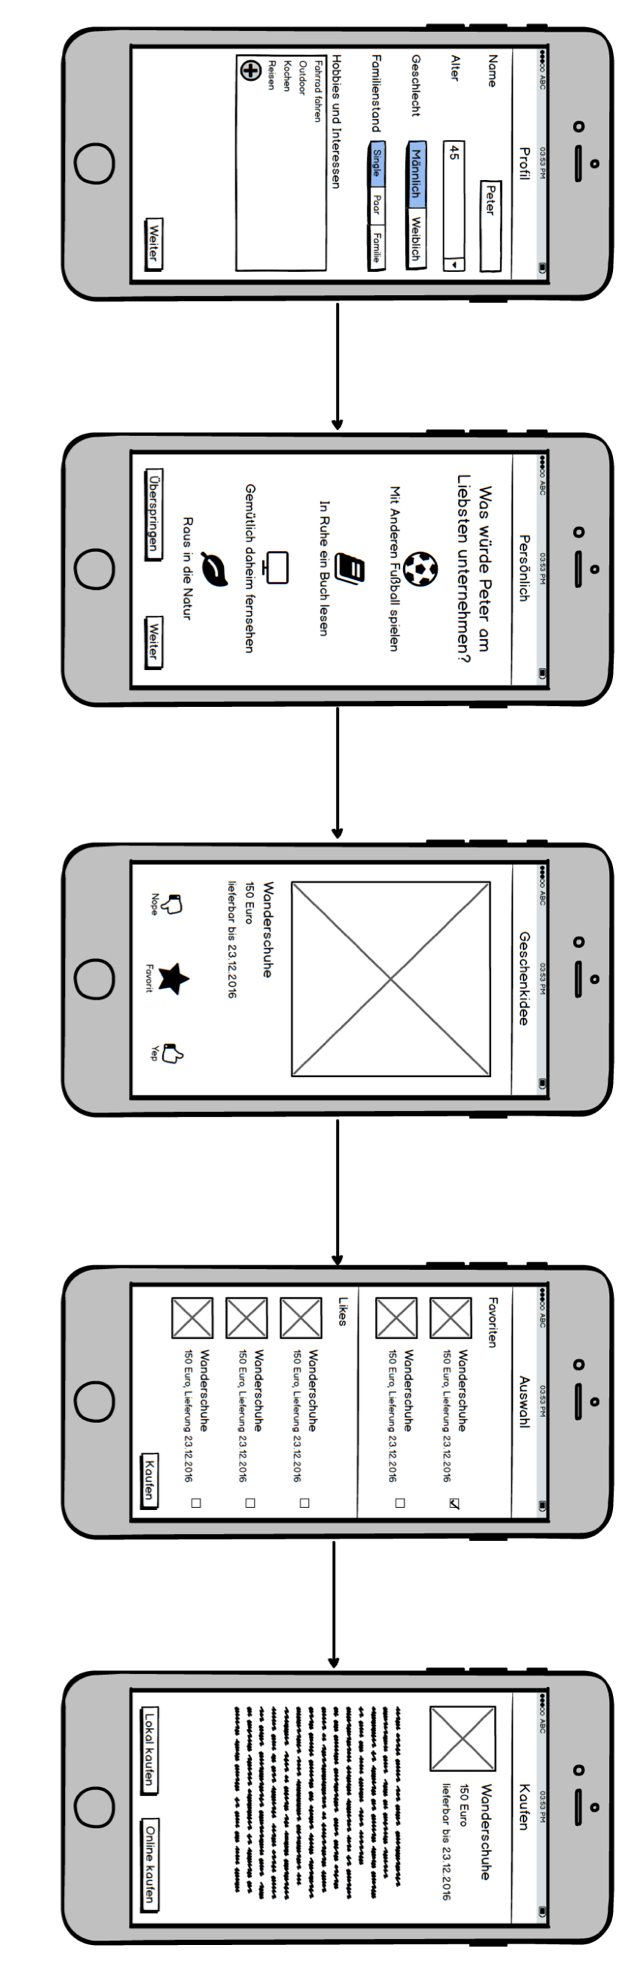
\includegraphics[height=0.83\paperheight]{prt1}}
    \caption{Swipe-App (Prototyp 1)}
    \label{fig:prt1}
\end{figure}

\begin{figure}[ht]
    \centering
      \makebox[\textwidth]{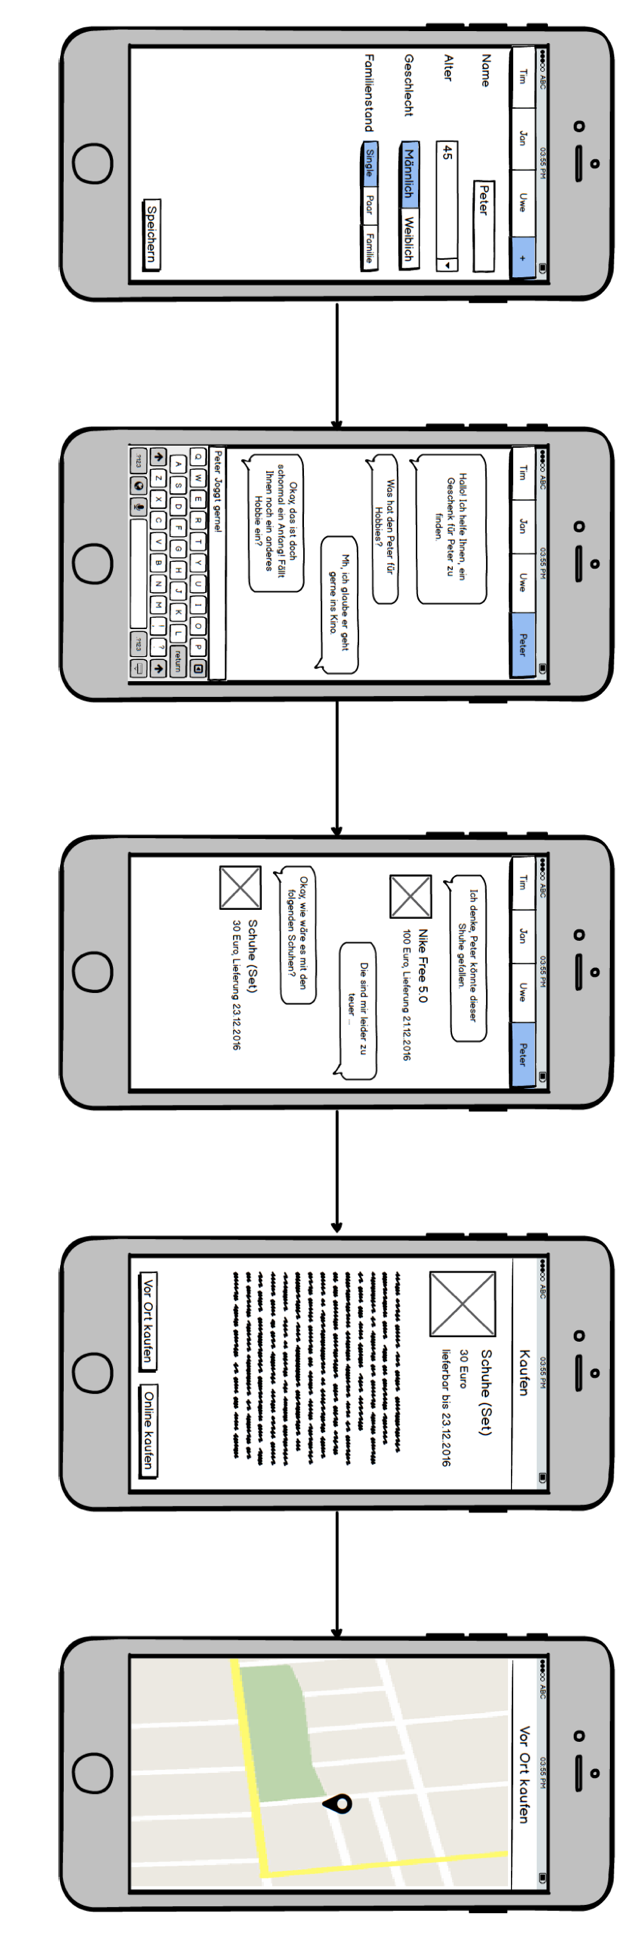
\includegraphics[height=0.83\paperheight]{prt2}}
    \caption{Chat-Bot (Prototyp 2)}
    \label{fig:prt2}
\end{figure}

\begin{figure}[ht]
    \centering
      \makebox[\textwidth]{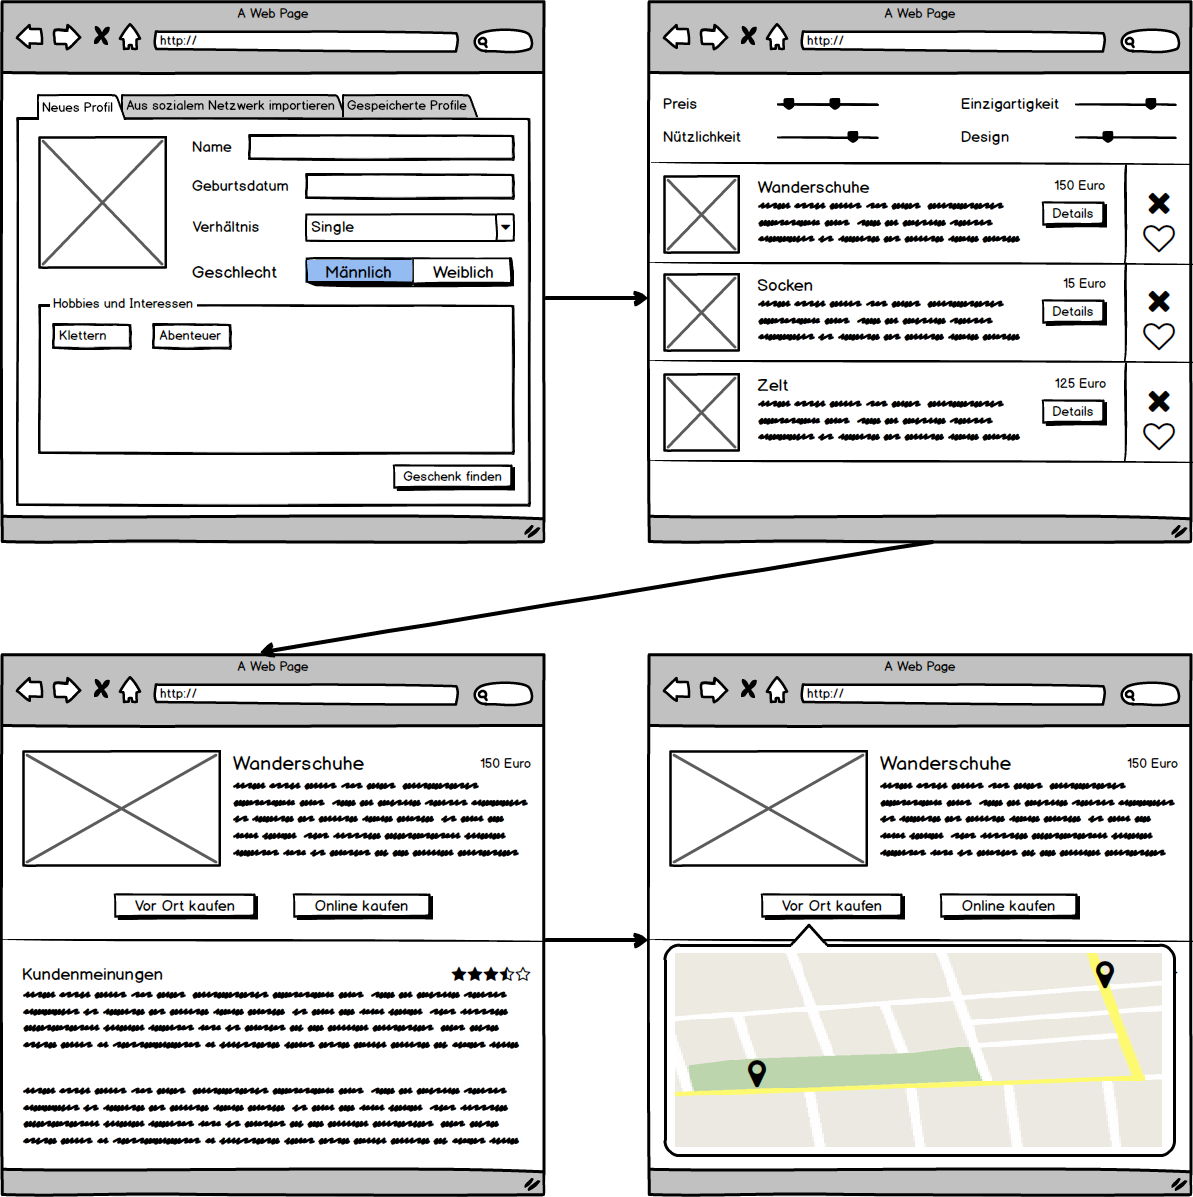
\includegraphics[width=0.83\paperwidth,height=0.65\paperheight]{prt3}}
    \caption{Webseite (Prototyp 3)}
    \label{fig:prt3}
\end{figure}

\begin{figure}[ht]
    \centering
      \makebox[\textwidth]{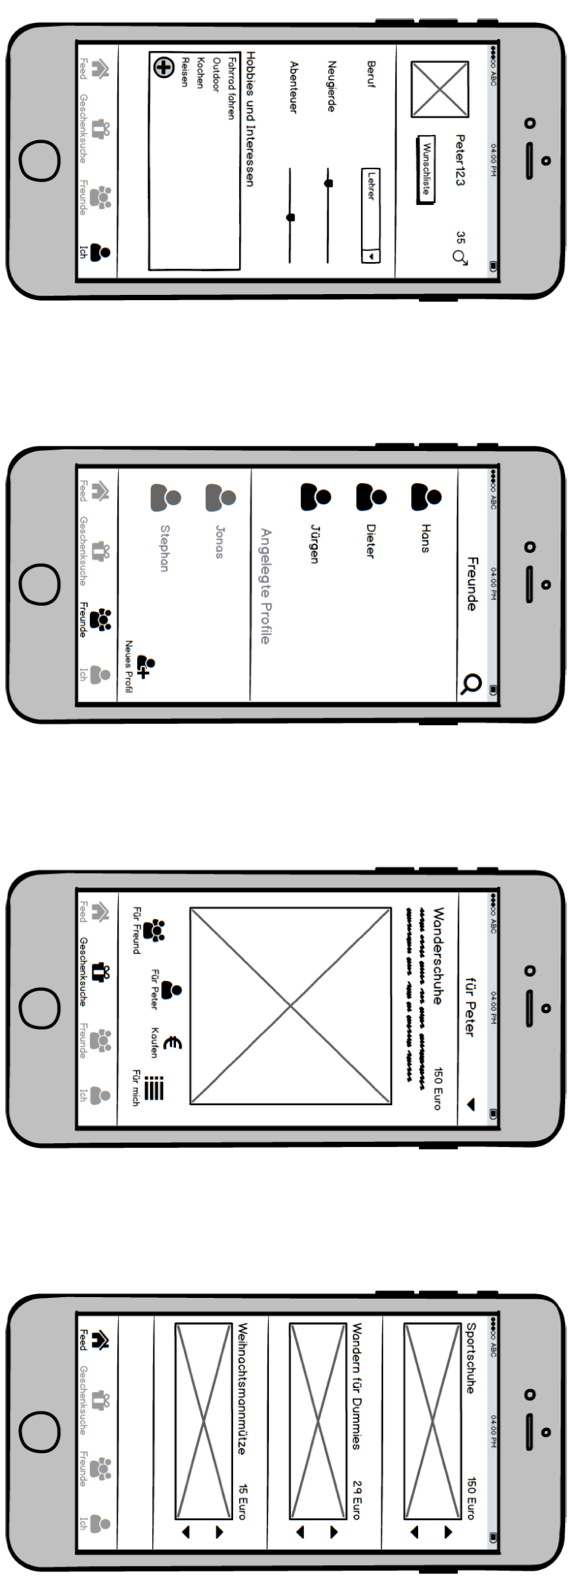
\includegraphics[height=0.8\paperheight]{prt4}}
    \caption{Soziales Netz (Prototyp 4)}
    \label{fig:prt4}
\end{figure}


\end{document}